%%%%%%%%%%%%%%%%%%%%%%%%%%%%%%%%%%%%%%%%%
% University Assignment Title Page 
% LaTeX Template
% Version 1.0 (27/12/12)
%
% This template has been downloaded from:
% http://www.LaTeXTemplates.com
%
% Original author:
% WikiBooks (http://en.wikibooks.org/wiki/LaTeX/Title_Creation)
%
% License:
% CC BY-NC-SA 3.0 (http://creativecommons.org/licenses/by-nc-sa/3.0/)
% 
% Instructions for using this template:
% This title page is capable of being compiled as is. This is not useful for 
% including it in another document. To do this, you have two options: 
%
% 1) Copy/paste everything between \begin{document} and \end{document} 
% starting at \begin{titlepage} and paste this into another LaTeX file where you 
% want your title page.
% OR
% 2) Remove everything outside the \begin{titlepage} and \end{titlepage} and 
% move this file to the same directory as the LaTeX file you wish to add it to. 
% Then add %%%%%%%%%%%%%%%%%%%%%%%%%%%%%%%%%%%%%%%%%
% University Assignment Title Page 
% LaTeX Template
% Version 1.0 (27/12/12)
%
% This template has been downloaded from:
% http://www.LaTeXTemplates.com
%
% Original author:
% WikiBooks (http://en.wikibooks.org/wiki/LaTeX/Title_Creation)
%
% License:
% CC BY-NC-SA 3.0 (http://creativecommons.org/licenses/by-nc-sa/3.0/)
% 
% Instructions for using this template:
% This title page is capable of being compiled as is. This is not useful for 
% including it in another document. To do this, you have two options: 
%
% 1) Copy/paste everything between \begin{document} and \end{document} 
% starting at \begin{titlepage} and paste this into another LaTeX file where you 
% want your title page.
% OR
% 2) Remove everything outside the \begin{titlepage} and \end{titlepage} and 
% move this file to the same directory as the LaTeX file you wish to add it to. 
% Then add %%%%%%%%%%%%%%%%%%%%%%%%%%%%%%%%%%%%%%%%%
% University Assignment Title Page 
% LaTeX Template
% Version 1.0 (27/12/12)
%
% This template has been downloaded from:
% http://www.LaTeXTemplates.com
%
% Original author:
% WikiBooks (http://en.wikibooks.org/wiki/LaTeX/Title_Creation)
%
% License:
% CC BY-NC-SA 3.0 (http://creativecommons.org/licenses/by-nc-sa/3.0/)
% 
% Instructions for using this template:
% This title page is capable of being compiled as is. This is not useful for 
% including it in another document. To do this, you have two options: 
%
% 1) Copy/paste everything between \begin{document} and \end{document} 
% starting at \begin{titlepage} and paste this into another LaTeX file where you 
% want your title page.
% OR
% 2) Remove everything outside the \begin{titlepage} and \end{titlepage} and 
% move this file to the same directory as the LaTeX file you wish to add it to. 
% Then add %%%%%%%%%%%%%%%%%%%%%%%%%%%%%%%%%%%%%%%%%
% University Assignment Title Page 
% LaTeX Template
% Version 1.0 (27/12/12)
%
% This template has been downloaded from:
% http://www.LaTeXTemplates.com
%
% Original author:
% WikiBooks (http://en.wikibooks.org/wiki/LaTeX/Title_Creation)
%
% License:
% CC BY-NC-SA 3.0 (http://creativecommons.org/licenses/by-nc-sa/3.0/)
% 
% Instructions for using this template:
% This title page is capable of being compiled as is. This is not useful for 
% including it in another document. To do this, you have two options: 
%
% 1) Copy/paste everything between \begin{document} and \end{document} 
% starting at \begin{titlepage} and paste this into another LaTeX file where you 
% want your title page.
% OR
% 2) Remove everything outside the \begin{titlepage} and \end{titlepage} and 
% move this file to the same directory as the LaTeX file you wish to add it to. 
% Then add \input{./title_page_1.tex} to your LaTeX file where you want your
% title page.
%
%%%%%%%%%%%%%%%%%%%%%%%%%%%%%%%%%%%%%%%%%

%-------------------------------------------------------------------------------
%	PACKAGES AND OTHER DOCUMENT CONFIGURATIONS
%-------------------------------------------------------------------------------

\documentclass{article}

\usepackage{amsmath}
\usepackage{amssymb} % Needed for certain math elements
\usepackage{clrscode3e} % Intro to Algorithms style pseudo-code
\usepackage{fancyhdr}
\usepackage{extramarks}
\usepackage{graphicx} % Required for the inclusion of images
\usepackage{enumerate}
\usepackage[parfill]{parskip} % Creates newline between paragraphs
\usepackage{rotating} % sideways table
\usepackage{caption}

% <paste>
%
% Homework Details
%   - Title
%   - Due date
%   - Class
%   - Section/Time
%   - Instructor
%   - Author
%

\newcommand{\hmwkTitle}{DAA Assignment}
\newcommand{\hmwkDueDate}{May 16, 2016}
\newcommand{\hmwkClass}{COMP3001}
\newcommand{\hmwkClassTime}{Section A}
\newcommand{\hmwkClassInstructor}{Professor Isaac Newton}
\newcommand{\hmwkAuthorName}{Chris Garland (15560955)}
%
% Basic Document Settings
%

\topmargin=-0.45in
\evensidemargin=0in
\oddsidemargin=0in
\textwidth=6.5in
\textheight=9.0in
\headsep=0.25in

\linespread{1.1}

\pagestyle{fancy}
\lhead{\hmwkAuthorName}
\chead{\hmwkClass: \hmwkTitle}
\rhead{\firstxmark}
\lfoot{\lastxmark}
\cfoot{\thepage}

\renewcommand\headrulewidth{0.4pt}
\renewcommand\footrulewidth{0.4pt}

\setlength\parindent{0pt}

%
% Create Problem Sections
%

\newcommand{\enterProblemHeader}[1]{
    \nobreak\extramarks{}{Question \arabic{#1} continued on next 
    page\ldots}\nobreak{}
    \nobreak\extramarks{Question \arabic{#1} (continued)}{Question \arabic{#1} 
    continued on next page \ldots}\nobreak{}
}

\newcommand{\exitProblemHeader}[1]{
    \nobreak\extramarks{Question \arabic{#1} (continued)}{Question \arabic{#1} 
    continued on next page\ldots}\nobreak{}
    \stepcounter{#1}
    \nobreak\extramarks{Question \arabic{#1}}{}\nobreak{}
}

\setcounter{secnumdepth}{0}
\newcounter{partCounter}
\newcounter{homeworkProblemCounter}
\setcounter{homeworkProblemCounter}{1}
\nobreak\extramarks{Question \arabic{homeworkProblemCounter}}{}\nobreak{}

%
% Homework Problem Environment
%
% This environment takes an optional argument. When given, it will adjust the
% problem counter. This is useful for when the problems given for your
% assignment aren't sequential. See the last 3 problems of this template for an
% example.
%
\newenvironment{homeworkProblem}[1][-1]{
    \ifnum#1>0
        \setcounter{homeworkProblemCounter}{#1}
    \fi
    \section{Question \arabic{homeworkProblemCounter}}
    \setcounter{partCounter}{1}
    \enterProblemHeader{homeworkProblemCounter}
}{
    \exitProblemHeader{homeworkProblemCounter}
}

% </paste>
\begin{document}
\setlength{\belowdisplayskip}{1.2cm}
\setlength{\belowdisplayshortskip}{1.0cm}

\begin{titlepage}

% Defines a new command for the horizontal lines, change thickness here
\newcommand{\HRule}{\rule{\linewidth}{0.5mm}} 


\center % Center everything on the page
 
%-------------------------------------------------------------------------------
%	HEADING SECTIONS
%-------------------------------------------------------------------------------
%
\includegraphics[scale=0.3]{Curtin1}\\[1.5cm]
\textsc{\LARGE Curtin University}\\[1.5cm] % Name of your university/college
\textsc{\Large Department of Computing}\\[0.5cm] % Major heading/course name
\textsc{\large COMP3001}\\[0.5cm] % Minor heading such as course title

%-------------------------------------------------------------------------------
%	TITLE SECTION
%-------------------------------------------------------------------------------

\HRule \\[0.4cm]
{ \huge \bfseries Design and Analysis of Algorithms Assignment}\\[0.4cm] % Title
\HRule \\[1.5cm]
 
%-------------------------------------------------------------------------------
%	AUTHOR SECTION
%-------------------------------------------------------------------------------

\begin{minipage}{0.4\textwidth}
\begin{flushleft} \large
\emph{Author: 15560955}\\
Chris \textsc{Garland} % Your name
\end{flushleft}
\end{minipage}
~
\begin{minipage}{0.4\textwidth}
\begin{flushright} \large
\emph{Lecturer:} \\
Dr. Sie Teng \textsc{Soh} % Supervisor's Name
\end{flushright}
\end{minipage}\\[4cm]

% If you don't want a supervisor, uncomment the two lines below and remove the section above
%\Large \emph{Author:}\\
%John \textsc{Smith}\\[3cm] % Your name

%-------------------------------------------------------------------------------
%	DATE SECTION
%-------------------------------------------------------------------------------

{\large \today}\\[3cm] % Date, change the \today to a set date if you want to be precise

%-------------------------------------------------------------------------------
%	LOGO SECTION
%-------------------------------------------------------------------------------

% Include a department/university logo - this will require the graphicx package

\includegraphics[scale=0.25]{Curtin2}
 
%-------------------------------------------------------------------------------

\vfill % Fill the rest of the page with whitespace

\end{titlepage}

%-------------------------------------------------------------------------------
% Question 1
%-------------------------------------------------------------------------------
\begin{homeworkProblem}
\begin{enumerate}[a)]
	\item \textbf{(10 marks).} Use the Master method to solve the following 
    recurrence function:
    	\begin{equation}
			T(n) = 3T(\sqrt[2]{n}) + \log_2 n
		\end{equation}
	\textbf{Solution:}
    \par
    Given the master theorem:
    \begin{equation}
		T(n) = aT(n/b) + f(n)
	\end{equation}
    \par 
    We can see that $a = 3$, $b = \sqrt{n}$ and $f(n) = \log_2 n$. As $b$ does not 
    conform to the master theorem, we will use a change of variable:
    \par 
    
    \textit{let}: $n = 2^{m} \therefore \log_2 n = m$ \\
    $\hspace*{1.87cm} \therefore \sqrt[2]{n} = 2^{m/2}$
    \begin{equation}
		T(2^{m}) = 3T(2^{m/2}) + m
	\end{equation}
    \par 
    Now, we perform another substitution \ldots
    \par
    \textit{let}: $T(2^{m}) = S(m)$\\
    \textit{let}: $T(2^{m/2}) = S(m/2)$
    \begin{equation}
		S(m) = 3S(m/2) + m
	\end{equation}
    \par 
    We now have a recurrence equation that conforms to the format of the Master 
    Theorem \ldots $a = 3$, $b = 2$ and $f(m) = m$. Lets compare $m^{\log_b a}$ with 
    $f(m)$ \ldots
    \par 
    $m^{\log_b a} = m^{\log_2 3} > f(m)$\\
    $f(m) = O(m^{\log_2 3 - \epsilon})$, where $\epsilon > 0$
    \par 
    By case 1 of Master Theorem:
    \begin{equation}
		S(m) = \Theta(m^{\log_2 3})
	\end{equation}
    We know that $S(m) = T(2^m)$ and $2^m = n \therefore$
    \begin{equation}
		T(n) = \Theta(m^{\log_2 3})
	\end{equation}
    Given that $m = \log_2 n$ \ldots
    \begin{equation}
    \begin{aligned}
		T(n) &= \Theta((\log_2 n)^{\log_2 3})\\
        &= \Theta(\log_2^{\log_2 3} n)
	\end{aligned}
	\end{equation}
    
    
\end{enumerate}
\end{homeworkProblem}

\clearpage

%-------------------------------------------------------------------------------
% Question 2
%-------------------------------------------------------------------------------
\begin{homeworkProblem}
Consider the following communication network that is represented by a weighted 
graph $G = (V, E)$ in which the non-negative number $r_{u,v}$ represents the 
\textit{operational probability} or \textit{reliability} of link 
$(u, v) \in E$ for $0 \leq r_{u,v} \leq 1.0$. Recall that a path $P_{a,b}$ is a 
sequence of links from a given source node $a$ to its destination node $b$. The 
reliability of a path (called \textit{path reliability}), $r_{a,b}$, is computed 
by multiplying the reliability of each link in path $P_{a,b}$. For example of 
path $P_{A,E} =$ (A, D, B, E) from source node A to destination node E is 
$R_{A,E} = (0.9 * 0.85 * 0.8) = 0.612$. We define \textit{the most reliable path} 
from a source node $s$ to a destination node $t$ as the path with the highest 
reliability among all possible paths form $s$ to $t$, i.e., the maximum 
$R_{s,t}$. \\[2cm]

\begin{figure}[h]
\begin{center}

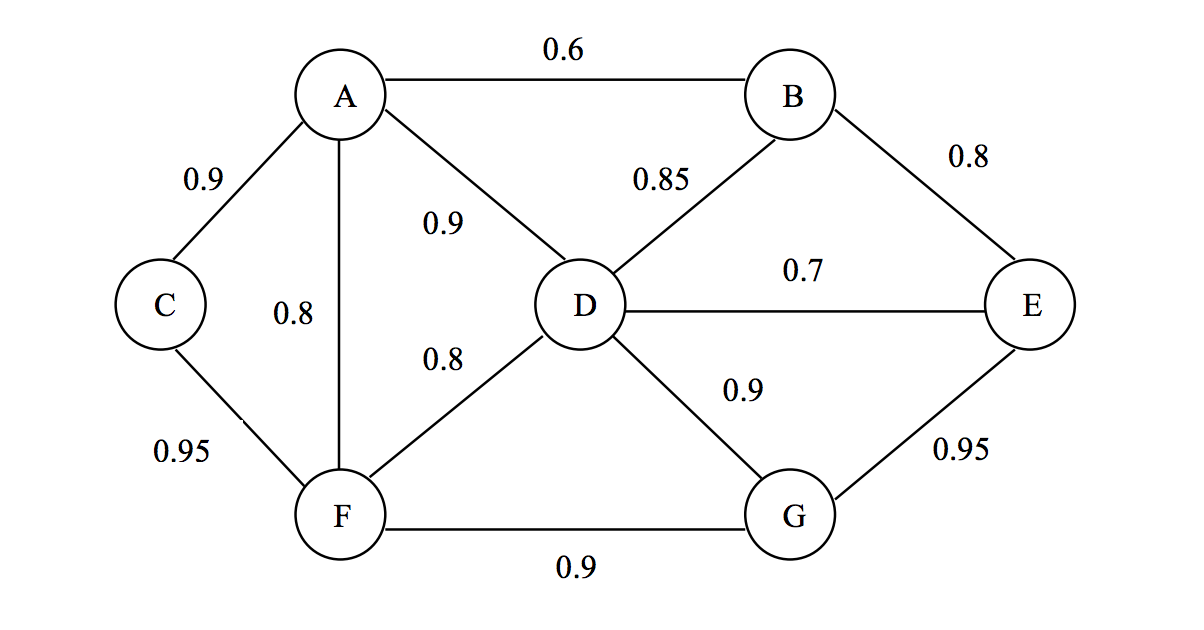
\includegraphics[scale=0.77]{Diag1}
\caption{Weighted graph representation of a communication network}

\end{center}
\end{figure}

\clearpage

\begin{enumerate}[a)]
	\item \textbf{(25 marks).} Design a \textit{greedy} algorithm that generates 
    the most reliable path from a source node $s$ to every destination node $t$ 
    in the network. 
    \par
	\textbf{Solution:}
    \par

    In this design we will modify Dijkstra's algorithm to \textit{greedily} 
    determine the most reliable path from a source node $s$ to every destination 
    node in the network. Original time complexity is maintained: 
    $O(|E| + |V|\log_2|V|)$ \ldots
    
    \begin{codebox}
    \Procname{$\proc{Dijkstra-Modified}(G, w, s)$}
    \li $\proc{Initialize-Single-Source}(G,s)$
    \li $S = \emptyset$
    \li $Q = \attribxx{G}{V}$
    \li \While $Q \neq \emptyset$
   	\li 	\Do
    		    $u = \proc{Extract-Max}(Q)$\>\>\>\>\>\>\Comment Modification
                \textit{from}: $u =$ \proc{Extract-Min}(Q)
    \li         $S = S\ \cup\ \{u\}$
    \li 	    \For each vertex $v \in \attrib{G}{Adj[u]}$
    \li             \Do
                        $\proc{Relax(u, v, w)}$
                    \End
            \End        
    \end{codebox}
    
    Line 1 initializes the $d$ and $\pi$ values as shown below. Line 2 initializes 
    the set $S$ to the empty set. Line 3 initializes the \textit{max-priority} 
    queue $Q$ to contain all the vertices in $V$. Each time through the 
    \textbf{while} loop of lines 4--8, line 5 extracts a vertex from $Q$ and line 
    6 adds it to $S$. Lines 7--8 relax each edge $(u, v)$ and updates the estimate 
    \attrib{v}{d} if the path reliability can be improved.
    
    \begin{codebox}
    \Procname{$\proc{Initialize-Single-Source}(G, s)$}
    \li \For each vertex $v \in \attribxx{G}{V}$
   	\li     \Do
    			$\attribxx{v}{d} = 0$\>\>\>\>\>\>\Comment Modification 
                \textit{from}: \attrib{v}{d} $= \infty$
    \li         $\attribxx{v}{\pi} = \const{nil}$\>\>\>\>\>\>\Comment $v$'s 
    												predecessor
            \End
    \li $\attribxx{s}{d} = 1$\>\>\>\>\>\>\>\Comment Modification \textit{from}: 
    \attrib{s}{d} $= 0$
    \end{codebox}
    
    We modify by initializing the \textit{reliability} attribute 
    $\attribxx{v}{d}$, of all $v \in V - \{s\}$ to $0$, which is a lower bound 
    on the weight/reliability of a path from source $s$ to $v$. We call 
    $\attribxx{v}{d}$ a path reliability estimate. The path-reliability attribute 
    $\attribxx{s}{d}$ of the source node $s$ is initialized to $1$ 
    (max reliability). 
    
    \begin{codebox}
    \Procname{$\proc{Relax}(u, v, w)$}
    \li \If $\attrib{v}{d} < \attrib{u}{d} \times w(u, v)$\>\>\>\>\>\>\>\Comment 
    		Modification \textit{from}: $\attrib{v}{d} > \attrib{u}{d} + w(u, v)$
    \li 	\Do
    			$\attrib{v}{d} = \attrib{u}{d} \times w(v, v)$\>\>\>\>\>\>\Comment
                Modification \textit{from}: $\attrib{v}{d} = \attrib{u}{d} +
                w(u, v)$
    \li 		$\attrib{v}{\pi} = u$\>\>\>\>\>\>\Comment $v$'s predecessor
    		\End
    \end{codebox}
    
    \begin{figure}[h]
		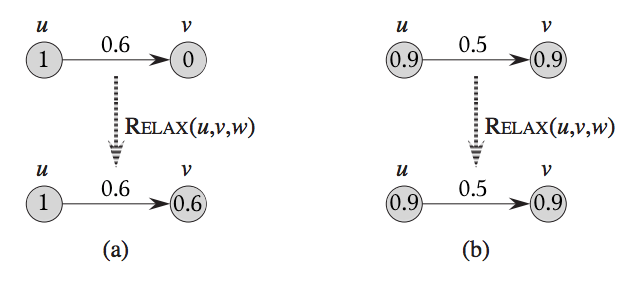
\includegraphics[scale=0.8]{Relax}
        \caption[caption]{\textbf{(a)} Because the value of $\attrib{v}{d} < 
        		 \attrib{u}{d} \times w(u, v)$ prior to relaxation, the value of 
                 \attrib{v}{d} is updated. 
                 \\\hspace*{1.53cm}\textbf{(b)} Here, $\attrib{v}{d} \geq 
                 \attrib{u}{d} \times w(u, v)$ before relaxation, and so 
                 \attrib{v}{d} remains unchanged. }
	\end{figure}
    
    \clearpage
    
    \item \textbf{(15 marks)}. Use your algorithm in part a) to generate the most 
    reliable path from node A to every other node in the given graph. List the 
    most reliable paths and their corresponding path reliabilities.
    \par
    \textbf{Solution:}
    \par
    \vspace*{7cm}
    \begin{center}
    \textit{On Next Page \ldots}
	\end{center}
%==============================================================================
\begin{sidewaystable}[ht]
\centering
\resizebox{\columnwidth}{!}{%
%\caption{My caption}
\label{my-label}
\begin{tabular}{ccccccccccc}
\textbf{Step \#} & \textbf{Unvisited($Q$)} & \textbf{Visited($S$)} & \textbf{Current($u$)} & \multicolumn{7}{l}{\textbf{Reliability of Path to Vertex($v$): (reliability{[}$s$-$v${]}, predecessor($\pi$))$_{iteration}$}} \\
\multicolumn{1}{l}{}                 & \multicolumn{1}{l}{}                      & \multicolumn{1}{l}{}                    & \multicolumn{1}{l}{}                    & \textbf{A($s$)}  & \textbf{B}   & \textbf{C}  & \textbf{D}  & \textbf{E}    & \textbf{F}   & \textbf{G}  \\
\textbf{Init}                        & \{A, B, C, D, E, F, G\}                   & \{-\}                                   & N/A                                     & (1, -)$_0$        & (0, -)$_0$    & (0, -)$_0$   & (0, -)$_0$   & (0, -)$_0$     & (0, -)$_0$    & (0, -)$_0$   \\
\textbf{1}                           & \{B, C, D, E, F, G\}                      & \{A\}                                   & A                                       & (1, -)$_0$        & (0.6, A)$_1$    & (0.9, A)$_1$   & (0.9, A)$_1$   & (0, -)$_0$     & (0.8, A)$_1$    & (0, -)$_0$   \\
\textbf{2}                           & \{B, D, E, F, G\}                         & \{A, C\}                                & C                                       & (1, -)$_2$        & (0.6, A)$_1$    & (0.9, A)$_1$   & (0.9, A)$_1$   & (0, -)$_0$     & (0.855, C)$_2$  & (0, -)$_0$   \\
\textbf{3}                           & \{B, E, F, G\}                            & \{A, C, D\}                             & D                                       & (1, -)$_3$        & (0.765, D)$_3$  & (0.9, A)$_1$   & (0.9, A)$_1$   & (0.63, D)$_3$    & (0.855, C)$_3$  & (0.81, D)$_3$  \\
\textbf{4}                           & \{B, E, G\}                               & \{A, C, D, F\}                          & F                                       & (1, -)$_4$        & (0.765, D)$_3$  & (0.9, A)$_4$   & (0.9, A)$_4$   & (0.63, D)$_3$    & (0.855, C)$_3$  & (0.81, D)$_3$  \\
\textbf{5}                           & \{B, E\}                                  & \{A, C, D, F, G\}                       & G                                       & (1, -)$_4$        & (0.765, D)$_3$  & (0.9, A)$_4$   & (0.9, A)$_5$   & (0.7695, G)$_5$  & (0.855, C)$_5$  & (0.81, D)$_3$  \\
\textbf{6}                           & \{B\}                                     & \{A, C, D, E, F, G\}                    & E                                       & (1, -)$_4$        & (0.765, D)$_6$  & (0.9, A)$_4$   & (0.9, A)$_6$   & (0.7695, G)$_5$  & (0.855, C)$_5$  & (0.81, D)$_6$  \\
\textbf{7}                           & \{-\}                                     & \{A, B, C, D, E, F, G\}                 & B                                       & (1, -)$_7$        & (0.765, D)$_6$  & (0.9, A)$_4$   & (0.9, A)$_7$   & (0.7695, G)$_7$  & (0.855, C)$_5$  & (0.81, D)$_6$ 
\end{tabular}
}%
\end{sidewaystable}
%===============================================================================
\end{enumerate}
\end{homeworkProblem}

\clearpage

%-------------------------------------------------------------------------------
% Question 3
%-------------------------------------------------------------------------------
\begin{homeworkProblem}
Consider an undirected graph $G = (V, E)$, where $V$ is a set of nodes and $E$ 
is a  set of links. As an example, consider the following graph, where each 
link is  labeled by a lower case letter, e.g., link $a$ connects nodes A and C. 
As defined  in Chapter 23 of the textbook (Introduction to Algorithms by Cormen, 
et al), a  cut $(S, V – S)$ is a partition of nodes in $V$. Further, a link 
$(u, v) \in E$ \textit{crosses} the cut $(S, V – S)$ if \textbf{either} node 
$u \in S$ and $v \in (V – S)$ \textbf{or} node $u \in (V – S)$ and  $v \in S$; 
i.e., one of its end points is in $S$ and the other is in  $V – S$. As an  
example, $S_1 = \{C\}$ and $S_2 = V - S_1 =$ {A, B, D, E, F, G} is a cut. 
The weight of a  cut is defined as the number of links \textbf{crossing} the cut. 
As an  example, the  weight of the cut $(S_1, S_2)$ is two; there are two 
crossing links in the cut. The \textbf{maximum cut} (called \textbf{Max-Cut}) is 
a cut with the \textbf{maximum weight}. The problem of finding a maximum cut in 
a graph is known as the \textbf{Max-Cut Problem}, a well known NP-complete 
problem. \\[2cm]

\begin{figure}[h]
\begin{center}

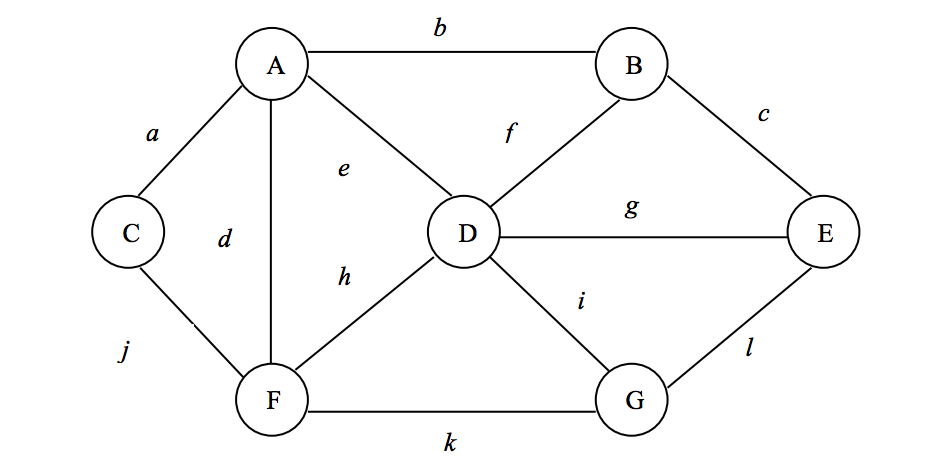
\includegraphics[scale=0.97]{Diag2}
\caption{Weighted graph representation of a communication network}

\end{center}
\end{figure}

\clearpage

\begin{enumerate}[a)]
	\item \textbf{(5 marks).} Generate all possible cuts in the given graph, and 
    determine its maximum cut.
    \par
	\textbf{Solution:}
    \par

	In order to determine the number of all possible cuts, we will use the formula \ldots 
    \begin{equation}
		2^n - 2
	\end{equation}
    Here we have $n$ as the number of vertices. This will give us the number of 
    \textit{all} possible combinations including the empty \textit{and} full sets. This is
    why we subtract $2$. This will give us the answer \ldots 
    
    \begin{equation}
    \begin{aligned}
		2^n - 2 &= 2^7 - 2\\
        &= 126
	\end{aligned}
	\end{equation}
    
    This is the number of all possible cuts. \\
    \par
    In the figure below will provide the \proc{Max-Cut} \ldots
    
    \vspace*{3cm}
    
	\begin{figure}[h]
	\begin{center}

	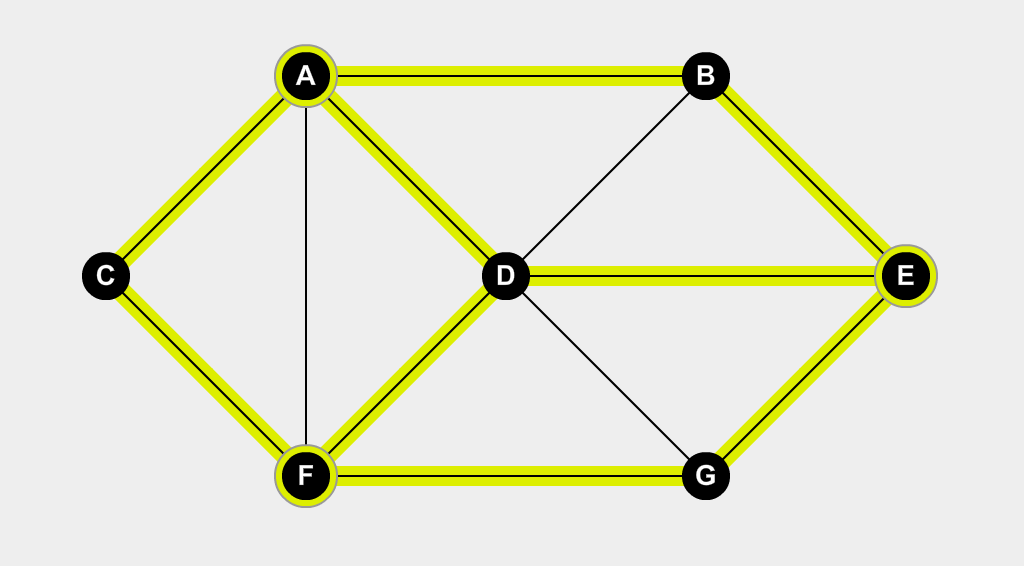
\includegraphics[scale=0.5]{max-cut}
	\caption{Max-Cut of graph illustrated in previous figure}

	\end{center}
	\end{figure}
    
    \clearpage

    \item \textbf{(20 marks)}. Design a \textit{greedy} algorithm to solve the 
    Max-Cut problem. As part of your solution, you must state your \textit{greedy 
    criteria}. Further, show your algorithm in a concise but clear pseudo-code. 
    You must explain in detail each line of the pseudo-code and show how to 
    implement the algorithm so that it has the best possible time complexity.
    \par
    \textbf{Solution:}
    \par
    
    In this design we follow the greedy approach of making the locally optimal choice at 
    each stage with the hope of finding a global optimum. the idea behind this algorithm
    is that we have two sets $S_1$ and $S_2$. $S_1$ will be initialized to contain the
    first vertex $v \in \attrib{G}{V}$ (A in this case). $S_2$ will be initialized to 
    $\attrib{G}{V} - S_1$ (all other vertices). Now we have $(S_1 = \{A\}, S_2 = 
    \{B, C, D, E, F, G\})$. Lets consider vertex A $\in S_1$. The number of cuts is
    determined by the number of adjacent vertices in $S_2$. In this case we have 4, 
    $\{B, C, D, F\}$. We will call this set \textit{external vertices}. Any vertices in 
    the same set, we will call \textit{internal vertices}. The algorithm runs through each 
    $v \in \attrib{G}{V}$ and determines whether the number of \textit{internal vertices}
    $\geq$ the number of \textit{external vertices} \textbf{\textit{(greedy criteria)}}. 
    If so, then swap sets and maintain a boolean value to be use as a loop terminator.
    Once there is no more improvement, we have our final cut.\\
    \par 
    \textbf{Input:} Graph (all vertices \attrib{G}{V}, adjacency list \attrib{G}{adj[u]})
    \\
    \textbf{Output:} \proc{Max-Cut}  

	\begin{codebox}
    \Procname{$\proc{Max-Cut}(G)$}
    \li $S_1 = 1st \in \attrib{G}{V}$
    \li $S_2 = \attribxx{G}{V} - S_1$
    \li \textbf{do} 
   	\li 	\Do
    		    improvement = \const{false}
    \li 	    \For each vertex $u \in \attrib{G}{V}$
    \li             \Do
                        \If (num $v \in \attrib{G}{adj[u]}$) $\in$ current set 
                        $\geq$\\ 
                        \hspace*{1.92cm}(num $v \in \attrib{G}{adj[u]}$) $\in$ 
                        other set
	\li						\Do
    							\proc{Swap-Sets$(u, S_1, S_2)$}
    \li                         improvement = \const{true}
    						\End
                    \End
            \End 
    \li \While improvement
    \li \Return $(S_1, S_2)$
    \end{codebox}
    
    Lines 1--2 initialize the sets. In this case, to $(\{A\}, \{B, C, D, E, F, G\})$. The
    \textbf{do} - \While loop on lines 3--9 will terminate if the boolean value on Line 4 
    is not adjusted to \const{true}. The \For loop on lines 5--8 will iterate over every 
    vertex $v \in \attrib{G}{V}$. The \If statement on line 6 is what makes this algorithm 
    greedy. \If number of \textit{internal vertices} $\geq$ number \textit{external 
    vertices} then swap sets and maintain bool value to keep the loop going. Finally when 
    there does not exist a vertex that has a greater number of \textit{internal vertices}, 
    Line 10 will \Return the max-cut. 
    
    \begin{codebox}
	\Procname{$\proc{Swap-Sets}(u)$}
    \li \If $\attrib{u}{currentSet} \isequal S_1$
    \li 	\Do 
    			$S_1 = S_1 - \{u\}$
    \li         $S_2 = S_2 \cup \{u\}$
    \li 		$\attrib{u}{currentSet} = S_2$
    		\End 
    \li \Else
    \li		\Do 
            	$S_2 = S_2 - \{u\}$
    \li         $S_1 = S_1 \cup \{u\}$
    \li 		$\attrib{u}{currentNode} = S_1$
    		\End 
	\end{codebox}

	\clearpage

    \item \textbf{(10 marks)}. Use your algorithm in part b) to generate the 
    Max-Cut of the given graph. Does your algorithm generate an optimal result? 
    \par
    \textbf{Solution:}
    \par 
	\vspace*{7cm}
    
    \begin{center}
    \textit{On Next Page} \ldots
	\end{center}

    \clearpage
        
  \vspace*{2cm}
  
    \begin{figure}[ht]
\centering
\begin{minipage}{.5\textwidth}
  \centering
  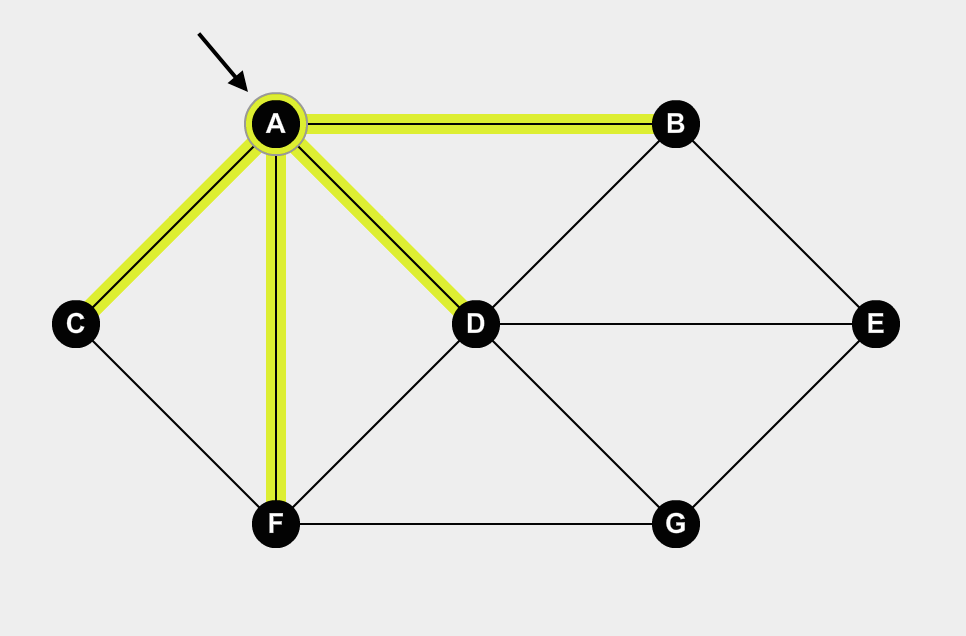
\includegraphics[width=.4\linewidth]{q3-a2}
  \captionof{figure}{$S_1 = \{A\}; S_2 = \{B, C, D, E, F, G\}$}
  \label{fig:test3}
\end{minipage}%
\begin{minipage}{.5\textwidth}
  \centering
  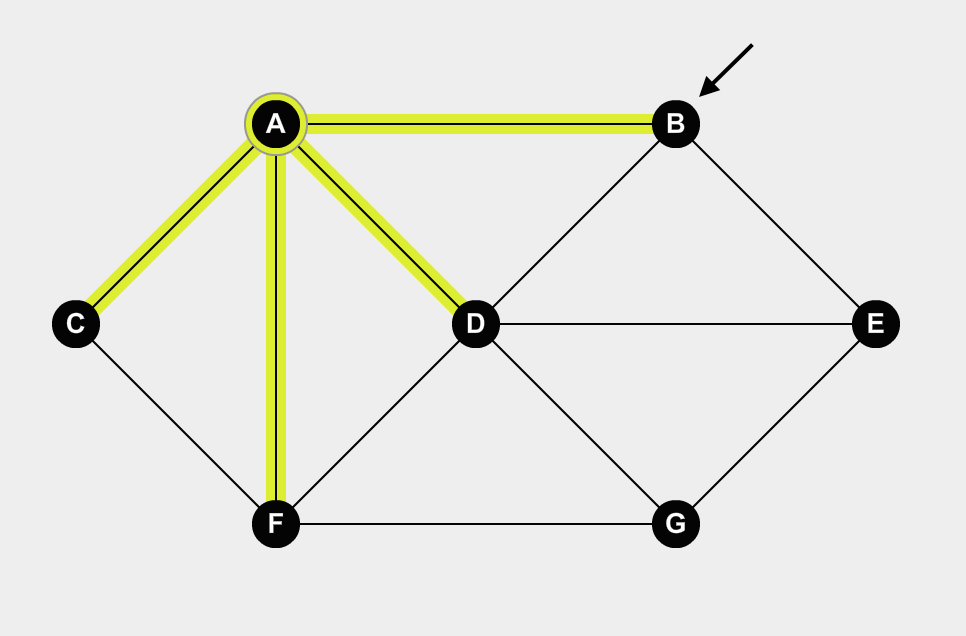
\includegraphics[width=.4\linewidth]{q3-b1}
  \captionof{figure}{Internal edges $\geq$ External edges}
  \label{fig:test4}
\end{minipage}
\end{figure}

\vspace*{3cm}

    \begin{figure}[ht]
\centering
\begin{minipage}{.5\textwidth}
  \centering
  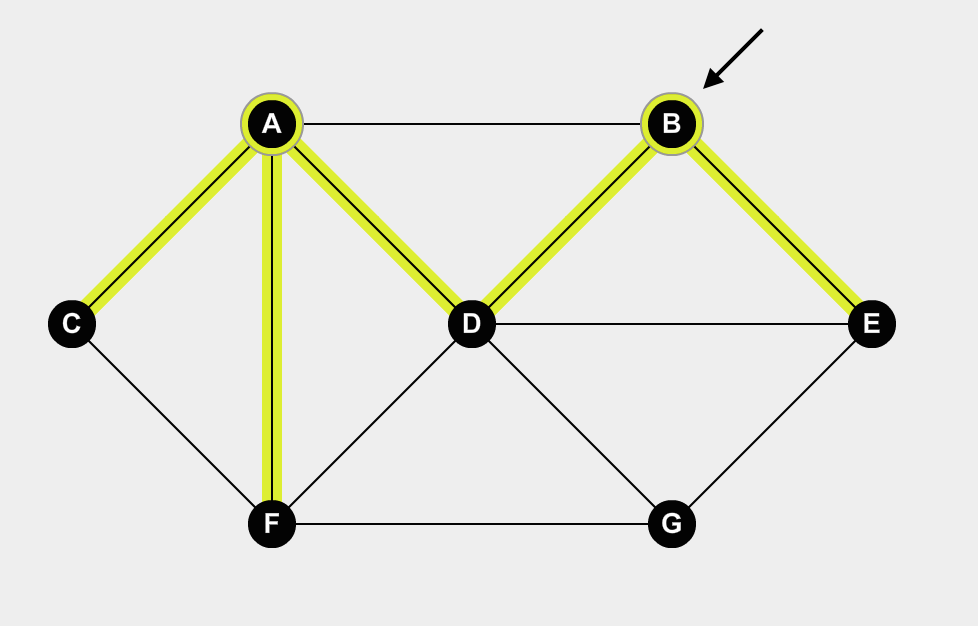
\includegraphics[width=.4\linewidth]{q3-b2}
  \captionof{figure}{$S_1 = \{A, B\}; S_2 = \{C, D, E, F, G\}$}
  \label{fig:test5}
\end{minipage}%
\begin{minipage}{.5\textwidth}
  \centering
  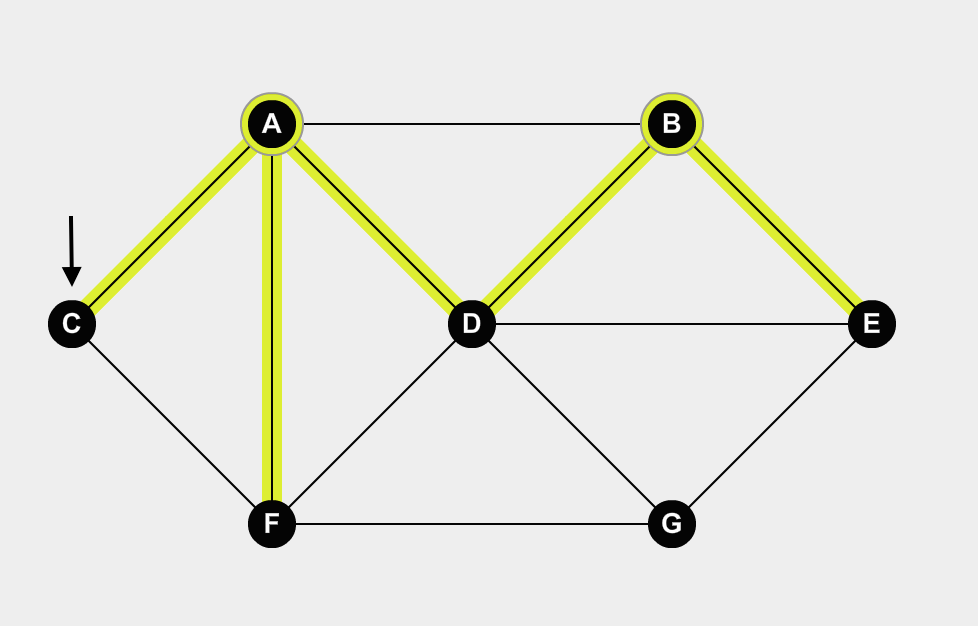
\includegraphics[width=.4\linewidth]{q3-c1}
  \captionof{figure}{Internal edges $\geq$ External edges}
  \label{fig:test6}
\end{minipage}
\end{figure}

\vspace*{3cm}

    \begin{figure}[ht]
\centering
\begin{minipage}{.5\textwidth}
  \centering
  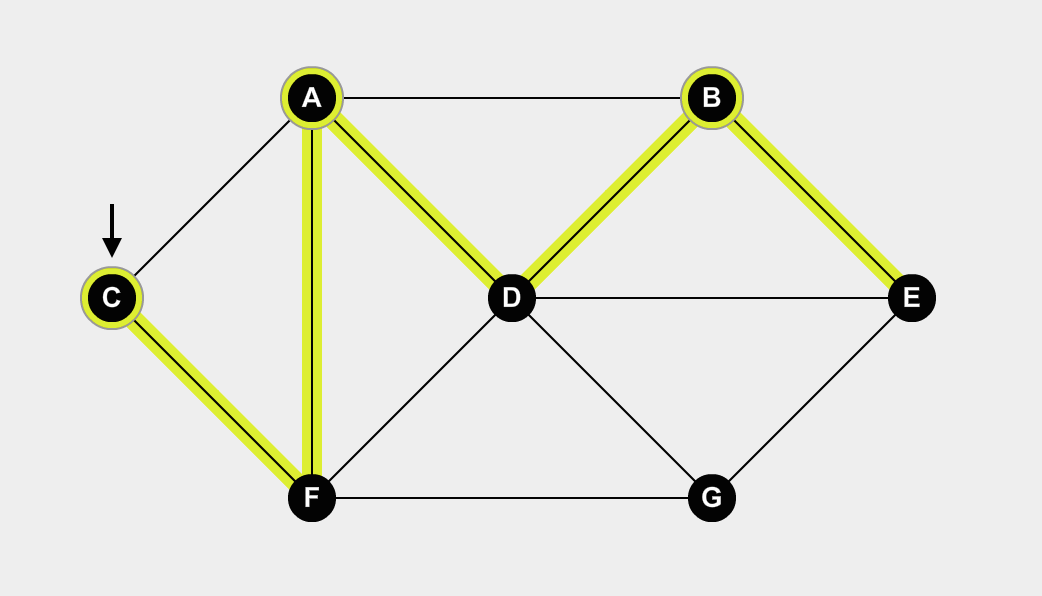
\includegraphics[width=.4\linewidth]{q3-c2}
  \captionof{figure}{$S_1 = \{A, B, C\}; S_2 = \{D, E, F, G\}$}
  \label{fig:test7}
\end{minipage}%
\begin{minipage}{.5\textwidth}
  \centering
  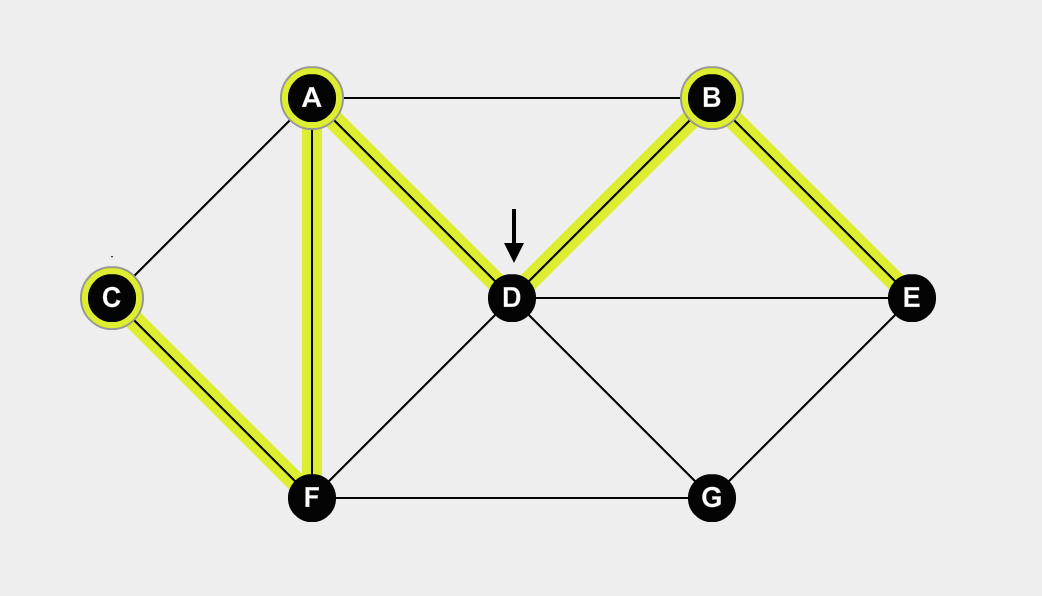
\includegraphics[width=.4\linewidth]{q3-d1}
  \captionof{figure}{Internal edges $\geq$ External edges}
  \label{fig:test8}
\end{minipage}
\end{figure}

    \begin{figure}[ht]
\centering
\begin{minipage}{.5\textwidth}
  \centering
  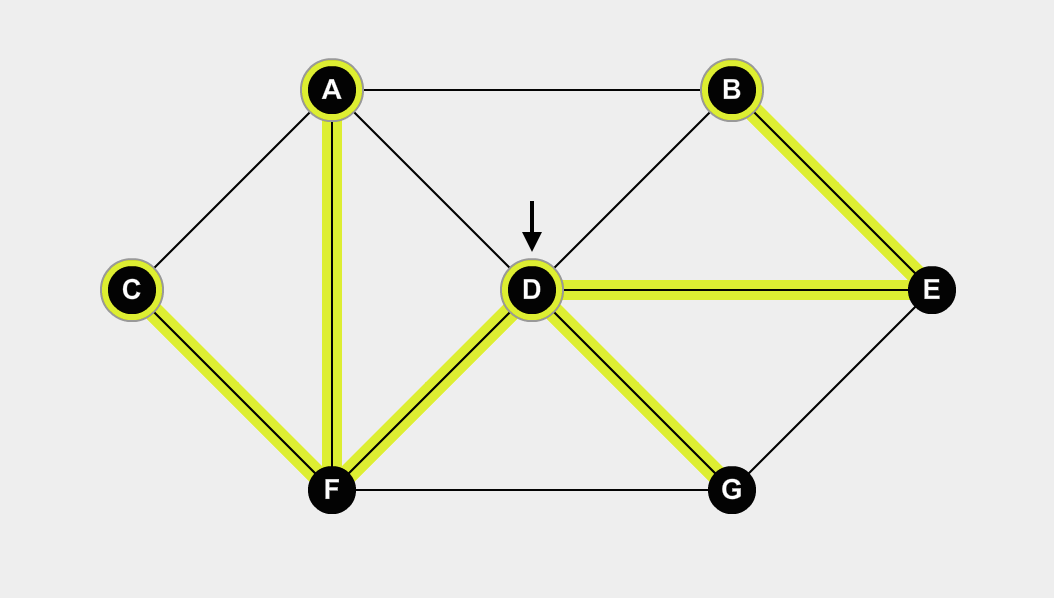
\includegraphics[width=.4\linewidth]{q3-d2}
  \captionof{figure}{$S_1 = \{A, B, C, D\}; S_2 = \{E, F, G\}$}
  \label{fig:test9}
\end{minipage}%
\begin{minipage}{.5\textwidth}
  \centering
  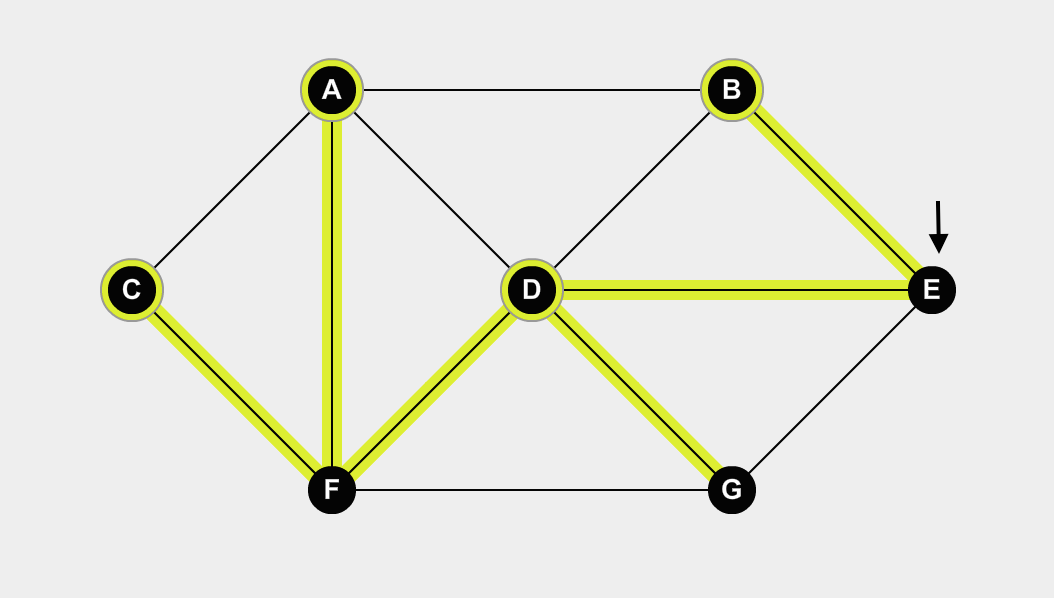
\includegraphics[width=.4\linewidth]{q3-e1}
  \captionof{figure}{Internal edges $\ngeq$ External edges}
  \label{fig:test10}
\end{minipage}
\end{figure}

    \begin{figure}[ht]
\centering
\begin{minipage}{.5\textwidth}
  \centering
  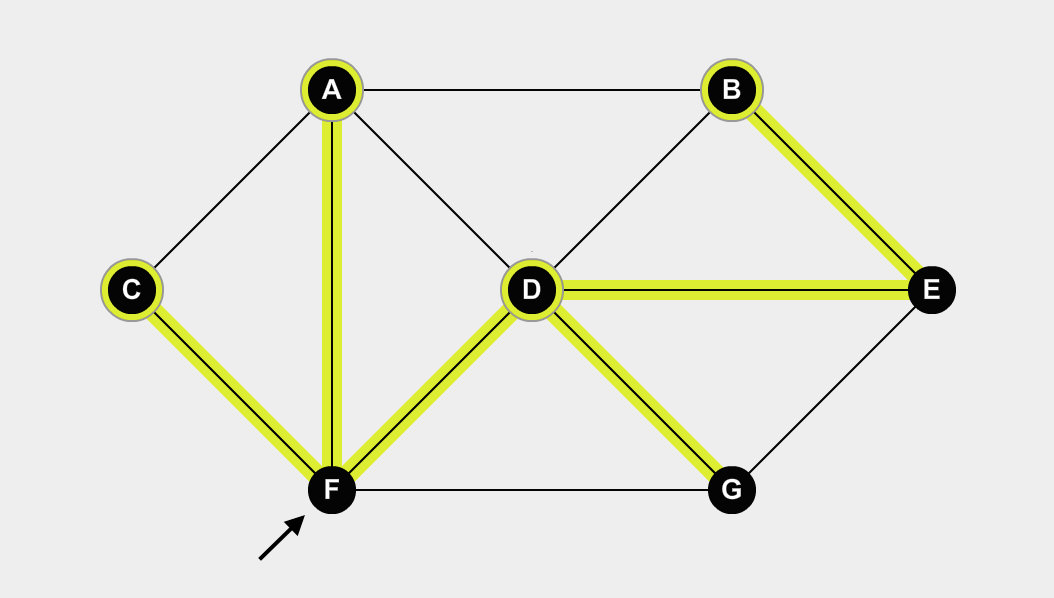
\includegraphics[width=.4\linewidth]{q3-f1}
  \captionof{figure}{Internal edges $\ngeq$ External edges}
  \label{fig:test11}
\end{minipage}%
\begin{minipage}{.5\textwidth}
  \centering
  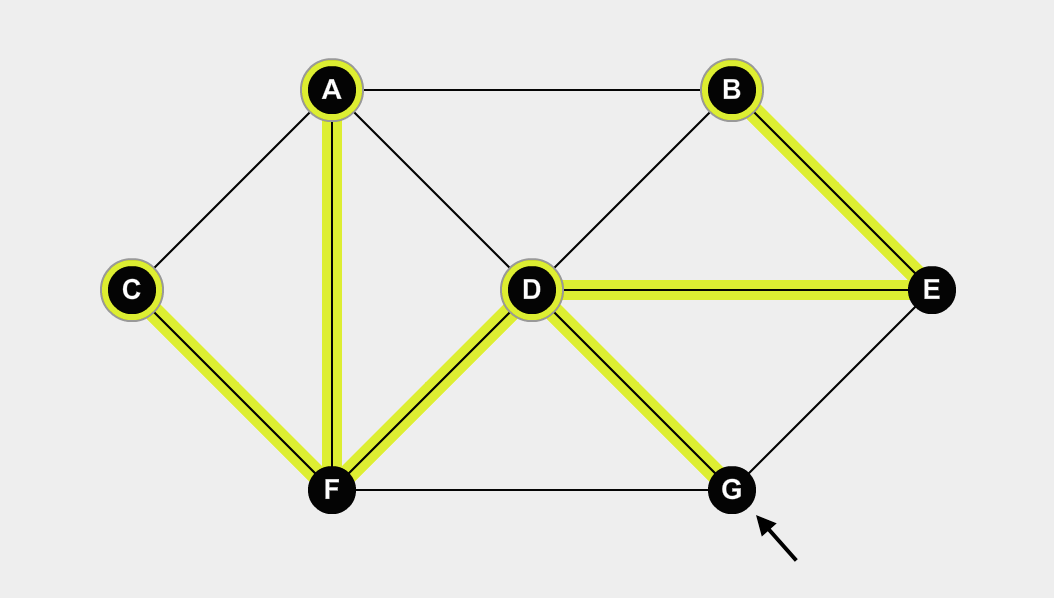
\includegraphics[width=.4\linewidth]{q3-g1}
  \captionof{figure}{Internal edges $\geq$ External edges}
  \label{fig:test12}
\end{minipage}
\end{figure}

    \begin{figure}[ht]
\centering
\begin{minipage}{.5\textwidth}
  \centering
  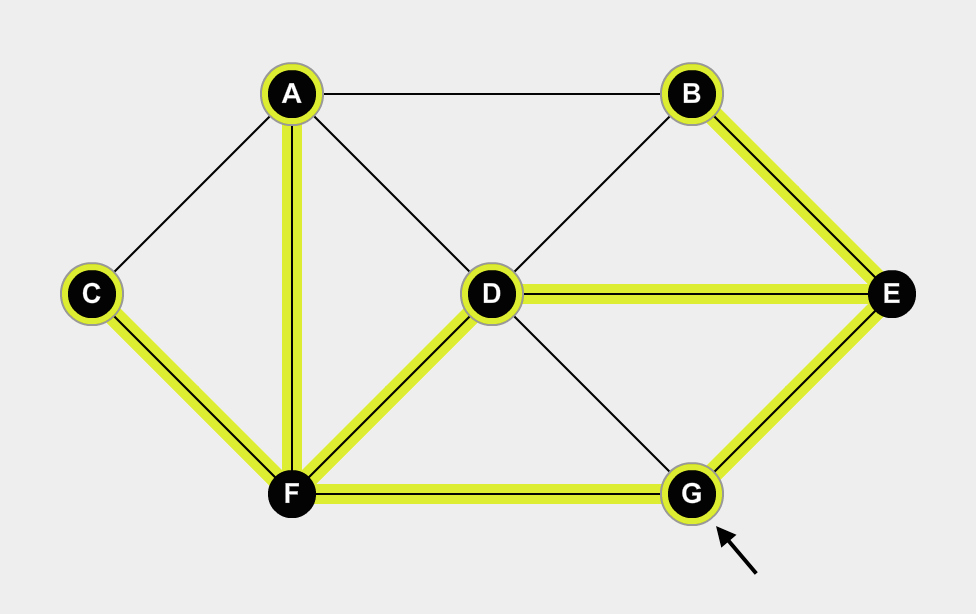
\includegraphics[width=.4\linewidth]{q3-g2}
  \captionof{figure}{$S_1 = \{A, B, C, D, G\}; S_2 = \{E, F\}$}
  \label{fig:test13}
\end{minipage}%
\begin{minipage}{.5\textwidth}
  \centering
  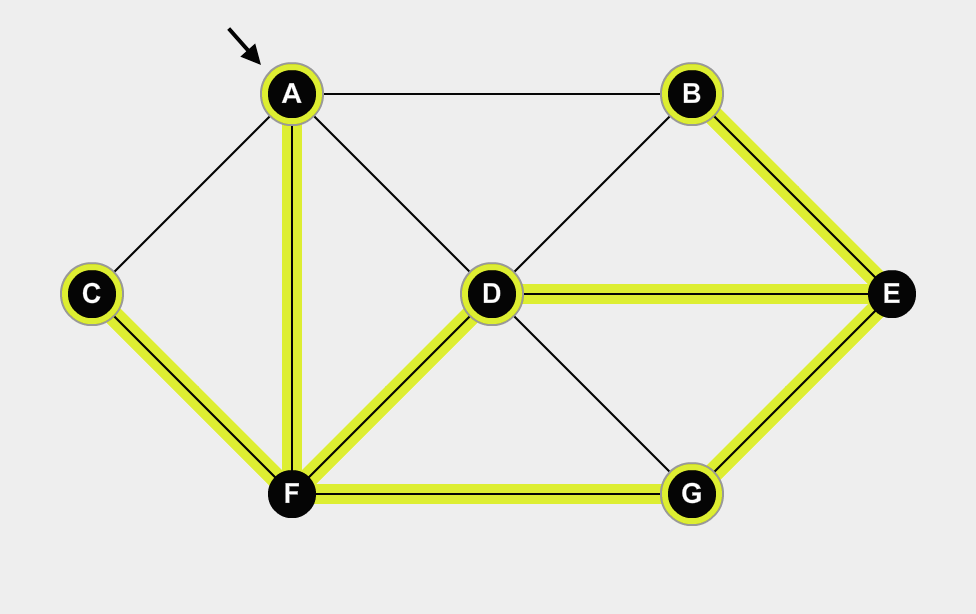
\includegraphics[width=.4\linewidth]{q3-a3}
  \captionof{figure}{Internal edges $\geq$ External edges}
  \label{fig:test14}
\end{minipage}
\end{figure}

	\begin{figure}[ht]
	\begin{center}

	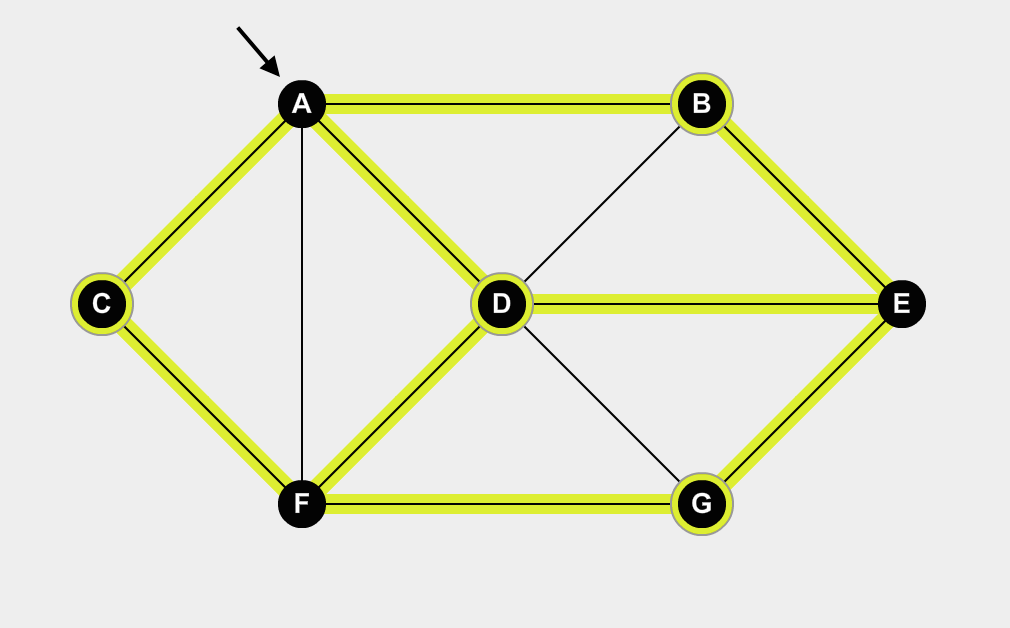
\includegraphics[scale=0.2]{q3-a4}
	\caption{$S_1 = \{B, C, D\}; S_2 = \{A, E, F\} = \proc{Max-Cut}$}

	\end{center}
	\end{figure}
    

\clearpage
    
	\item \textbf{(5 marks)}. Give a counter example to show that your greedy 
    algorithm does not always generate an optimal result.
    \par
    \textbf{Solution:}
    \par
    
    The algorithm may not produce the optimal result in the case of a bipartite graph. 
\end{enumerate}

\end{homeworkProblem}

\end{document}














 to your LaTeX file where you want your
% title page.
%
%%%%%%%%%%%%%%%%%%%%%%%%%%%%%%%%%%%%%%%%%

%-------------------------------------------------------------------------------
%	PACKAGES AND OTHER DOCUMENT CONFIGURATIONS
%-------------------------------------------------------------------------------

\documentclass{article}

\usepackage{amsmath}
\usepackage{amssymb} % Needed for certain math elements
\usepackage{clrscode3e} % Intro to Algorithms style pseudo-code
\usepackage{fancyhdr}
\usepackage{extramarks}
\usepackage{graphicx} % Required for the inclusion of images
\usepackage{enumerate}
\usepackage[parfill]{parskip} % Creates newline between paragraphs
\usepackage{rotating} % sideways table
\usepackage{caption}

% <paste>
%
% Homework Details
%   - Title
%   - Due date
%   - Class
%   - Section/Time
%   - Instructor
%   - Author
%

\newcommand{\hmwkTitle}{DAA Assignment}
\newcommand{\hmwkDueDate}{May 16, 2016}
\newcommand{\hmwkClass}{COMP3001}
\newcommand{\hmwkClassTime}{Section A}
\newcommand{\hmwkClassInstructor}{Professor Isaac Newton}
\newcommand{\hmwkAuthorName}{Chris Garland (15560955)}
%
% Basic Document Settings
%

\topmargin=-0.45in
\evensidemargin=0in
\oddsidemargin=0in
\textwidth=6.5in
\textheight=9.0in
\headsep=0.25in

\linespread{1.1}

\pagestyle{fancy}
\lhead{\hmwkAuthorName}
\chead{\hmwkClass: \hmwkTitle}
\rhead{\firstxmark}
\lfoot{\lastxmark}
\cfoot{\thepage}

\renewcommand\headrulewidth{0.4pt}
\renewcommand\footrulewidth{0.4pt}

\setlength\parindent{0pt}

%
% Create Problem Sections
%

\newcommand{\enterProblemHeader}[1]{
    \nobreak\extramarks{}{Question \arabic{#1} continued on next 
    page\ldots}\nobreak{}
    \nobreak\extramarks{Question \arabic{#1} (continued)}{Question \arabic{#1} 
    continued on next page \ldots}\nobreak{}
}

\newcommand{\exitProblemHeader}[1]{
    \nobreak\extramarks{Question \arabic{#1} (continued)}{Question \arabic{#1} 
    continued on next page\ldots}\nobreak{}
    \stepcounter{#1}
    \nobreak\extramarks{Question \arabic{#1}}{}\nobreak{}
}

\setcounter{secnumdepth}{0}
\newcounter{partCounter}
\newcounter{homeworkProblemCounter}
\setcounter{homeworkProblemCounter}{1}
\nobreak\extramarks{Question \arabic{homeworkProblemCounter}}{}\nobreak{}

%
% Homework Problem Environment
%
% This environment takes an optional argument. When given, it will adjust the
% problem counter. This is useful for when the problems given for your
% assignment aren't sequential. See the last 3 problems of this template for an
% example.
%
\newenvironment{homeworkProblem}[1][-1]{
    \ifnum#1>0
        \setcounter{homeworkProblemCounter}{#1}
    \fi
    \section{Question \arabic{homeworkProblemCounter}}
    \setcounter{partCounter}{1}
    \enterProblemHeader{homeworkProblemCounter}
}{
    \exitProblemHeader{homeworkProblemCounter}
}

% </paste>
\begin{document}
\setlength{\belowdisplayskip}{1.2cm}
\setlength{\belowdisplayshortskip}{1.0cm}

\begin{titlepage}

% Defines a new command for the horizontal lines, change thickness here
\newcommand{\HRule}{\rule{\linewidth}{0.5mm}} 


\center % Center everything on the page
 
%-------------------------------------------------------------------------------
%	HEADING SECTIONS
%-------------------------------------------------------------------------------
%
\includegraphics[scale=0.3]{Curtin1}\\[1.5cm]
\textsc{\LARGE Curtin University}\\[1.5cm] % Name of your university/college
\textsc{\Large Department of Computing}\\[0.5cm] % Major heading/course name
\textsc{\large COMP3001}\\[0.5cm] % Minor heading such as course title

%-------------------------------------------------------------------------------
%	TITLE SECTION
%-------------------------------------------------------------------------------

\HRule \\[0.4cm]
{ \huge \bfseries Design and Analysis of Algorithms Assignment}\\[0.4cm] % Title
\HRule \\[1.5cm]
 
%-------------------------------------------------------------------------------
%	AUTHOR SECTION
%-------------------------------------------------------------------------------

\begin{minipage}{0.4\textwidth}
\begin{flushleft} \large
\emph{Author: 15560955}\\
Chris \textsc{Garland} % Your name
\end{flushleft}
\end{minipage}
~
\begin{minipage}{0.4\textwidth}
\begin{flushright} \large
\emph{Lecturer:} \\
Dr. Sie Teng \textsc{Soh} % Supervisor's Name
\end{flushright}
\end{minipage}\\[4cm]

% If you don't want a supervisor, uncomment the two lines below and remove the section above
%\Large \emph{Author:}\\
%John \textsc{Smith}\\[3cm] % Your name

%-------------------------------------------------------------------------------
%	DATE SECTION
%-------------------------------------------------------------------------------

{\large \today}\\[3cm] % Date, change the \today to a set date if you want to be precise

%-------------------------------------------------------------------------------
%	LOGO SECTION
%-------------------------------------------------------------------------------

% Include a department/university logo - this will require the graphicx package

\includegraphics[scale=0.25]{Curtin2}
 
%-------------------------------------------------------------------------------

\vfill % Fill the rest of the page with whitespace

\end{titlepage}

%-------------------------------------------------------------------------------
% Question 1
%-------------------------------------------------------------------------------
\begin{homeworkProblem}
\begin{enumerate}[a)]
	\item \textbf{(10 marks).} Use the Master method to solve the following 
    recurrence function:
    	\begin{equation}
			T(n) = 3T(\sqrt[2]{n}) + \log_2 n
		\end{equation}
	\textbf{Solution:}
    \par
    Given the master theorem:
    \begin{equation}
		T(n) = aT(n/b) + f(n)
	\end{equation}
    \par 
    We can see that $a = 3$, $b = \sqrt{n}$ and $f(n) = \log_2 n$. As $b$ does not 
    conform to the master theorem, we will use a change of variable:
    \par 
    
    \textit{let}: $n = 2^{m} \therefore \log_2 n = m$ \\
    $\hspace*{1.87cm} \therefore \sqrt[2]{n} = 2^{m/2}$
    \begin{equation}
		T(2^{m}) = 3T(2^{m/2}) + m
	\end{equation}
    \par 
    Now, we perform another substitution \ldots
    \par
    \textit{let}: $T(2^{m}) = S(m)$\\
    \textit{let}: $T(2^{m/2}) = S(m/2)$
    \begin{equation}
		S(m) = 3S(m/2) + m
	\end{equation}
    \par 
    We now have a recurrence equation that conforms to the format of the Master 
    Theorem \ldots $a = 3$, $b = 2$ and $f(m) = m$. Lets compare $m^{\log_b a}$ with 
    $f(m)$ \ldots
    \par 
    $m^{\log_b a} = m^{\log_2 3} > f(m)$\\
    $f(m) = O(m^{\log_2 3 - \epsilon})$, where $\epsilon > 0$
    \par 
    By case 1 of Master Theorem:
    \begin{equation}
		S(m) = \Theta(m^{\log_2 3})
	\end{equation}
    We know that $S(m) = T(2^m)$ and $2^m = n \therefore$
    \begin{equation}
		T(n) = \Theta(m^{\log_2 3})
	\end{equation}
    Given that $m = \log_2 n$ \ldots
    \begin{equation}
    \begin{aligned}
		T(n) &= \Theta((\log_2 n)^{\log_2 3})\\
        &= \Theta(\log_2^{\log_2 3} n)
	\end{aligned}
	\end{equation}
    
    
\end{enumerate}
\end{homeworkProblem}

\clearpage

%-------------------------------------------------------------------------------
% Question 2
%-------------------------------------------------------------------------------
\begin{homeworkProblem}
Consider the following communication network that is represented by a weighted 
graph $G = (V, E)$ in which the non-negative number $r_{u,v}$ represents the 
\textit{operational probability} or \textit{reliability} of link 
$(u, v) \in E$ for $0 \leq r_{u,v} \leq 1.0$. Recall that a path $P_{a,b}$ is a 
sequence of links from a given source node $a$ to its destination node $b$. The 
reliability of a path (called \textit{path reliability}), $r_{a,b}$, is computed 
by multiplying the reliability of each link in path $P_{a,b}$. For example of 
path $P_{A,E} =$ (A, D, B, E) from source node A to destination node E is 
$R_{A,E} = (0.9 * 0.85 * 0.8) = 0.612$. We define \textit{the most reliable path} 
from a source node $s$ to a destination node $t$ as the path with the highest 
reliability among all possible paths form $s$ to $t$, i.e., the maximum 
$R_{s,t}$. \\[2cm]

\begin{figure}[h]
\begin{center}

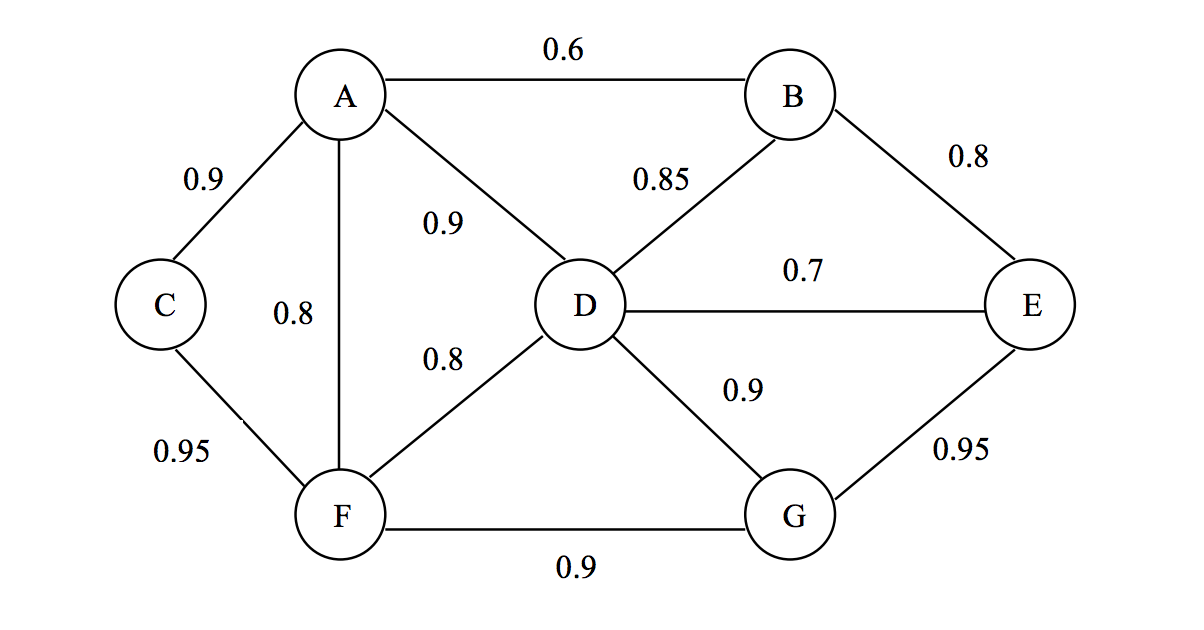
\includegraphics[scale=0.77]{Diag1}
\caption{Weighted graph representation of a communication network}

\end{center}
\end{figure}

\clearpage

\begin{enumerate}[a)]
	\item \textbf{(25 marks).} Design a \textit{greedy} algorithm that generates 
    the most reliable path from a source node $s$ to every destination node $t$ 
    in the network. 
    \par
	\textbf{Solution:}
    \par

    In this design we will modify Dijkstra's algorithm to \textit{greedily} 
    determine the most reliable path from a source node $s$ to every destination 
    node in the network. Original time complexity is maintained: 
    $O(|E| + |V|\log_2|V|)$ \ldots
    
    \begin{codebox}
    \Procname{$\proc{Dijkstra-Modified}(G, w, s)$}
    \li $\proc{Initialize-Single-Source}(G,s)$
    \li $S = \emptyset$
    \li $Q = \attribxx{G}{V}$
    \li \While $Q \neq \emptyset$
   	\li 	\Do
    		    $u = \proc{Extract-Max}(Q)$\>\>\>\>\>\>\Comment Modification
                \textit{from}: $u =$ \proc{Extract-Min}(Q)
    \li         $S = S\ \cup\ \{u\}$
    \li 	    \For each vertex $v \in \attrib{G}{Adj[u]}$
    \li             \Do
                        $\proc{Relax(u, v, w)}$
                    \End
            \End        
    \end{codebox}
    
    Line 1 initializes the $d$ and $\pi$ values as shown below. Line 2 initializes 
    the set $S$ to the empty set. Line 3 initializes the \textit{max-priority} 
    queue $Q$ to contain all the vertices in $V$. Each time through the 
    \textbf{while} loop of lines 4--8, line 5 extracts a vertex from $Q$ and line 
    6 adds it to $S$. Lines 7--8 relax each edge $(u, v)$ and updates the estimate 
    \attrib{v}{d} if the path reliability can be improved.
    
    \begin{codebox}
    \Procname{$\proc{Initialize-Single-Source}(G, s)$}
    \li \For each vertex $v \in \attribxx{G}{V}$
   	\li     \Do
    			$\attribxx{v}{d} = 0$\>\>\>\>\>\>\Comment Modification 
                \textit{from}: \attrib{v}{d} $= \infty$
    \li         $\attribxx{v}{\pi} = \const{nil}$\>\>\>\>\>\>\Comment $v$'s 
    												predecessor
            \End
    \li $\attribxx{s}{d} = 1$\>\>\>\>\>\>\>\Comment Modification \textit{from}: 
    \attrib{s}{d} $= 0$
    \end{codebox}
    
    We modify by initializing the \textit{reliability} attribute 
    $\attribxx{v}{d}$, of all $v \in V - \{s\}$ to $0$, which is a lower bound 
    on the weight/reliability of a path from source $s$ to $v$. We call 
    $\attribxx{v}{d}$ a path reliability estimate. The path-reliability attribute 
    $\attribxx{s}{d}$ of the source node $s$ is initialized to $1$ 
    (max reliability). 
    
    \begin{codebox}
    \Procname{$\proc{Relax}(u, v, w)$}
    \li \If $\attrib{v}{d} < \attrib{u}{d} \times w(u, v)$\>\>\>\>\>\>\>\Comment 
    		Modification \textit{from}: $\attrib{v}{d} > \attrib{u}{d} + w(u, v)$
    \li 	\Do
    			$\attrib{v}{d} = \attrib{u}{d} \times w(v, v)$\>\>\>\>\>\>\Comment
                Modification \textit{from}: $\attrib{v}{d} = \attrib{u}{d} +
                w(u, v)$
    \li 		$\attrib{v}{\pi} = u$\>\>\>\>\>\>\Comment $v$'s predecessor
    		\End
    \end{codebox}
    
    \begin{figure}[h]
		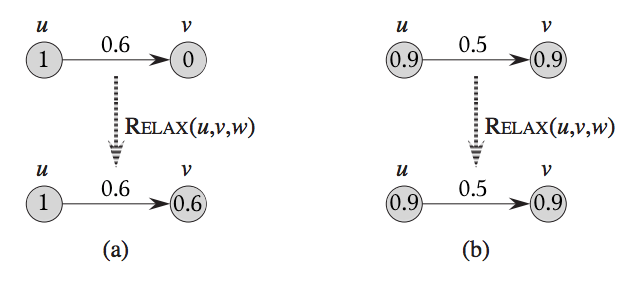
\includegraphics[scale=0.8]{Relax}
        \caption[caption]{\textbf{(a)} Because the value of $\attrib{v}{d} < 
        		 \attrib{u}{d} \times w(u, v)$ prior to relaxation, the value of 
                 \attrib{v}{d} is updated. 
                 \\\hspace*{1.53cm}\textbf{(b)} Here, $\attrib{v}{d} \geq 
                 \attrib{u}{d} \times w(u, v)$ before relaxation, and so 
                 \attrib{v}{d} remains unchanged. }
	\end{figure}
    
    \clearpage
    
    \item \textbf{(15 marks)}. Use your algorithm in part a) to generate the most 
    reliable path from node A to every other node in the given graph. List the 
    most reliable paths and their corresponding path reliabilities.
    \par
    \textbf{Solution:}
    \par
    \vspace*{7cm}
    \begin{center}
    \textit{On Next Page \ldots}
	\end{center}
%==============================================================================
\begin{sidewaystable}[ht]
\centering
\resizebox{\columnwidth}{!}{%
%\caption{My caption}
\label{my-label}
\begin{tabular}{ccccccccccc}
\textbf{Step \#} & \textbf{Unvisited($Q$)} & \textbf{Visited($S$)} & \textbf{Current($u$)} & \multicolumn{7}{l}{\textbf{Reliability of Path to Vertex($v$): (reliability{[}$s$-$v${]}, predecessor($\pi$))$_{iteration}$}} \\
\multicolumn{1}{l}{}                 & \multicolumn{1}{l}{}                      & \multicolumn{1}{l}{}                    & \multicolumn{1}{l}{}                    & \textbf{A($s$)}  & \textbf{B}   & \textbf{C}  & \textbf{D}  & \textbf{E}    & \textbf{F}   & \textbf{G}  \\
\textbf{Init}                        & \{A, B, C, D, E, F, G\}                   & \{-\}                                   & N/A                                     & (1, -)$_0$        & (0, -)$_0$    & (0, -)$_0$   & (0, -)$_0$   & (0, -)$_0$     & (0, -)$_0$    & (0, -)$_0$   \\
\textbf{1}                           & \{B, C, D, E, F, G\}                      & \{A\}                                   & A                                       & (1, -)$_0$        & (0.6, A)$_1$    & (0.9, A)$_1$   & (0.9, A)$_1$   & (0, -)$_0$     & (0.8, A)$_1$    & (0, -)$_0$   \\
\textbf{2}                           & \{B, D, E, F, G\}                         & \{A, C\}                                & C                                       & (1, -)$_2$        & (0.6, A)$_1$    & (0.9, A)$_1$   & (0.9, A)$_1$   & (0, -)$_0$     & (0.855, C)$_2$  & (0, -)$_0$   \\
\textbf{3}                           & \{B, E, F, G\}                            & \{A, C, D\}                             & D                                       & (1, -)$_3$        & (0.765, D)$_3$  & (0.9, A)$_1$   & (0.9, A)$_1$   & (0.63, D)$_3$    & (0.855, C)$_3$  & (0.81, D)$_3$  \\
\textbf{4}                           & \{B, E, G\}                               & \{A, C, D, F\}                          & F                                       & (1, -)$_4$        & (0.765, D)$_3$  & (0.9, A)$_4$   & (0.9, A)$_4$   & (0.63, D)$_3$    & (0.855, C)$_3$  & (0.81, D)$_3$  \\
\textbf{5}                           & \{B, E\}                                  & \{A, C, D, F, G\}                       & G                                       & (1, -)$_4$        & (0.765, D)$_3$  & (0.9, A)$_4$   & (0.9, A)$_5$   & (0.7695, G)$_5$  & (0.855, C)$_5$  & (0.81, D)$_3$  \\
\textbf{6}                           & \{B\}                                     & \{A, C, D, E, F, G\}                    & E                                       & (1, -)$_4$        & (0.765, D)$_6$  & (0.9, A)$_4$   & (0.9, A)$_6$   & (0.7695, G)$_5$  & (0.855, C)$_5$  & (0.81, D)$_6$  \\
\textbf{7}                           & \{-\}                                     & \{A, B, C, D, E, F, G\}                 & B                                       & (1, -)$_7$        & (0.765, D)$_6$  & (0.9, A)$_4$   & (0.9, A)$_7$   & (0.7695, G)$_7$  & (0.855, C)$_5$  & (0.81, D)$_6$ 
\end{tabular}
}%
\end{sidewaystable}
%===============================================================================
\end{enumerate}
\end{homeworkProblem}

\clearpage

%-------------------------------------------------------------------------------
% Question 3
%-------------------------------------------------------------------------------
\begin{homeworkProblem}
Consider an undirected graph $G = (V, E)$, where $V$ is a set of nodes and $E$ 
is a  set of links. As an example, consider the following graph, where each 
link is  labeled by a lower case letter, e.g., link $a$ connects nodes A and C. 
As defined  in Chapter 23 of the textbook (Introduction to Algorithms by Cormen, 
et al), a  cut $(S, V – S)$ is a partition of nodes in $V$. Further, a link 
$(u, v) \in E$ \textit{crosses} the cut $(S, V – S)$ if \textbf{either} node 
$u \in S$ and $v \in (V – S)$ \textbf{or} node $u \in (V – S)$ and  $v \in S$; 
i.e., one of its end points is in $S$ and the other is in  $V – S$. As an  
example, $S_1 = \{C\}$ and $S_2 = V - S_1 =$ {A, B, D, E, F, G} is a cut. 
The weight of a  cut is defined as the number of links \textbf{crossing} the cut. 
As an  example, the  weight of the cut $(S_1, S_2)$ is two; there are two 
crossing links in the cut. The \textbf{maximum cut} (called \textbf{Max-Cut}) is 
a cut with the \textbf{maximum weight}. The problem of finding a maximum cut in 
a graph is known as the \textbf{Max-Cut Problem}, a well known NP-complete 
problem. \\[2cm]

\begin{figure}[h]
\begin{center}

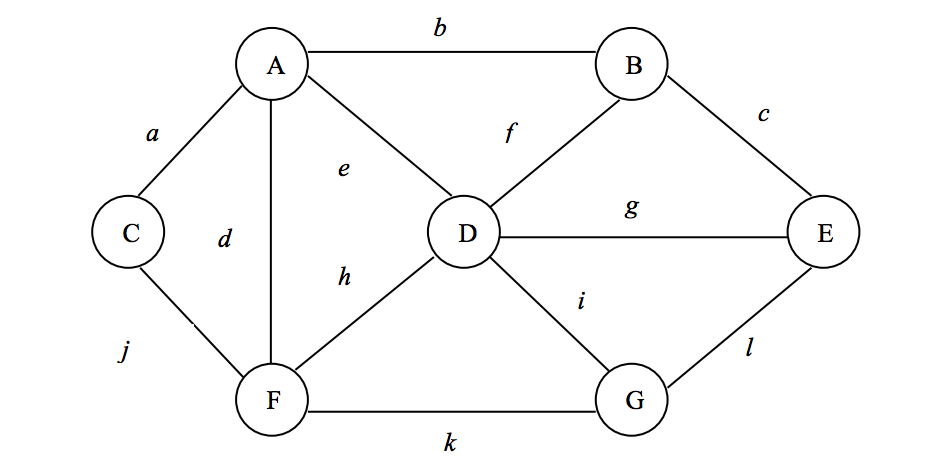
\includegraphics[scale=0.97]{Diag2}
\caption{Weighted graph representation of a communication network}

\end{center}
\end{figure}

\clearpage

\begin{enumerate}[a)]
	\item \textbf{(5 marks).} Generate all possible cuts in the given graph, and 
    determine its maximum cut.
    \par
	\textbf{Solution:}
    \par

	In order to determine the number of all possible cuts, we will use the formula \ldots 
    \begin{equation}
		2^n - 2
	\end{equation}
    Here we have $n$ as the number of vertices. This will give us the number of 
    \textit{all} possible combinations including the empty \textit{and} full sets. This is
    why we subtract $2$. This will give us the answer \ldots 
    
    \begin{equation}
    \begin{aligned}
		2^n - 2 &= 2^7 - 2\\
        &= 126
	\end{aligned}
	\end{equation}
    
    This is the number of all possible cuts. \\
    \par
    In the figure below will provide the \proc{Max-Cut} \ldots
    
    \vspace*{3cm}
    
	\begin{figure}[h]
	\begin{center}

	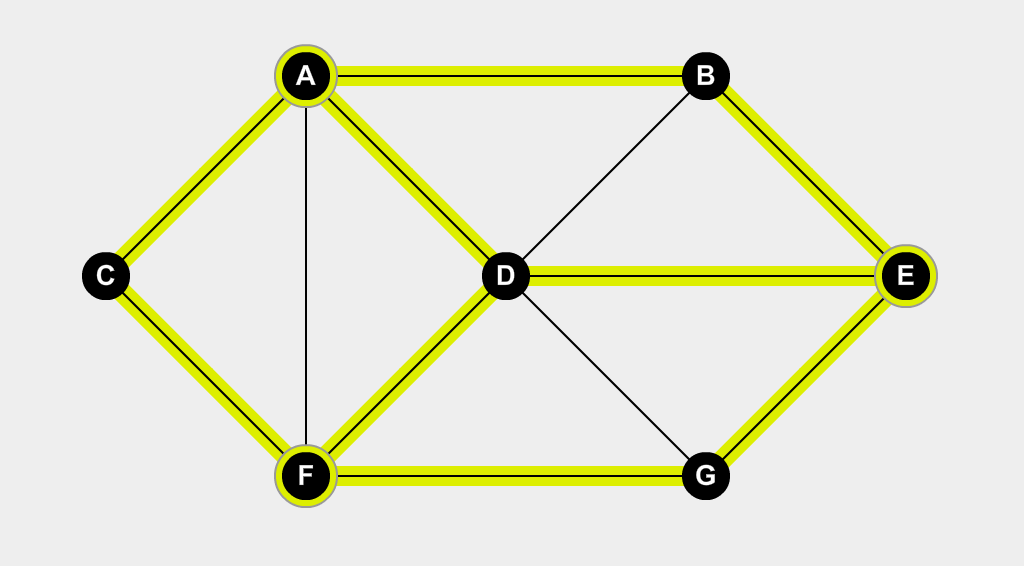
\includegraphics[scale=0.5]{max-cut}
	\caption{Max-Cut of graph illustrated in previous figure}

	\end{center}
	\end{figure}
    
    \clearpage

    \item \textbf{(20 marks)}. Design a \textit{greedy} algorithm to solve the 
    Max-Cut problem. As part of your solution, you must state your \textit{greedy 
    criteria}. Further, show your algorithm in a concise but clear pseudo-code. 
    You must explain in detail each line of the pseudo-code and show how to 
    implement the algorithm so that it has the best possible time complexity.
    \par
    \textbf{Solution:}
    \par
    
    In this design we follow the greedy approach of making the locally optimal choice at 
    each stage with the hope of finding a global optimum. the idea behind this algorithm
    is that we have two sets $S_1$ and $S_2$. $S_1$ will be initialized to contain the
    first vertex $v \in \attrib{G}{V}$ (A in this case). $S_2$ will be initialized to 
    $\attrib{G}{V} - S_1$ (all other vertices). Now we have $(S_1 = \{A\}, S_2 = 
    \{B, C, D, E, F, G\})$. Lets consider vertex A $\in S_1$. The number of cuts is
    determined by the number of adjacent vertices in $S_2$. In this case we have 4, 
    $\{B, C, D, F\}$. We will call this set \textit{external vertices}. Any vertices in 
    the same set, we will call \textit{internal vertices}. The algorithm runs through each 
    $v \in \attrib{G}{V}$ and determines whether the number of \textit{internal vertices}
    $\geq$ the number of \textit{external vertices} \textbf{\textit{(greedy criteria)}}. 
    If so, then swap sets and maintain a boolean value to be use as a loop terminator.
    Once there is no more improvement, we have our final cut.\\
    \par 
    \textbf{Input:} Graph (all vertices \attrib{G}{V}, adjacency list \attrib{G}{adj[u]})
    \\
    \textbf{Output:} \proc{Max-Cut}  

	\begin{codebox}
    \Procname{$\proc{Max-Cut}(G)$}
    \li $S_1 = 1st \in \attrib{G}{V}$
    \li $S_2 = \attribxx{G}{V} - S_1$
    \li \textbf{do} 
   	\li 	\Do
    		    improvement = \const{false}
    \li 	    \For each vertex $u \in \attrib{G}{V}$
    \li             \Do
                        \If (num $v \in \attrib{G}{adj[u]}$) $\in$ current set 
                        $\geq$\\ 
                        \hspace*{1.92cm}(num $v \in \attrib{G}{adj[u]}$) $\in$ 
                        other set
	\li						\Do
    							\proc{Swap-Sets$(u, S_1, S_2)$}
    \li                         improvement = \const{true}
    						\End
                    \End
            \End 
    \li \While improvement
    \li \Return $(S_1, S_2)$
    \end{codebox}
    
    Lines 1--2 initialize the sets. In this case, to $(\{A\}, \{B, C, D, E, F, G\})$. The
    \textbf{do} - \While loop on lines 3--9 will terminate if the boolean value on Line 4 
    is not adjusted to \const{true}. The \For loop on lines 5--8 will iterate over every 
    vertex $v \in \attrib{G}{V}$. The \If statement on line 6 is what makes this algorithm 
    greedy. \If number of \textit{internal vertices} $\geq$ number \textit{external 
    vertices} then swap sets and maintain bool value to keep the loop going. Finally when 
    there does not exist a vertex that has a greater number of \textit{internal vertices}, 
    Line 10 will \Return the max-cut. 
    
    \begin{codebox}
	\Procname{$\proc{Swap-Sets}(u)$}
    \li \If $\attrib{u}{currentSet} \isequal S_1$
    \li 	\Do 
    			$S_1 = S_1 - \{u\}$
    \li         $S_2 = S_2 \cup \{u\}$
    \li 		$\attrib{u}{currentSet} = S_2$
    		\End 
    \li \Else
    \li		\Do 
            	$S_2 = S_2 - \{u\}$
    \li         $S_1 = S_1 \cup \{u\}$
    \li 		$\attrib{u}{currentNode} = S_1$
    		\End 
	\end{codebox}

	\clearpage

    \item \textbf{(10 marks)}. Use your algorithm in part b) to generate the 
    Max-Cut of the given graph. Does your algorithm generate an optimal result? 
    \par
    \textbf{Solution:}
    \par 
	\vspace*{7cm}
    
    \begin{center}
    \textit{On Next Page} \ldots
	\end{center}

    \clearpage
        
  \vspace*{2cm}
  
    \begin{figure}[ht]
\centering
\begin{minipage}{.5\textwidth}
  \centering
  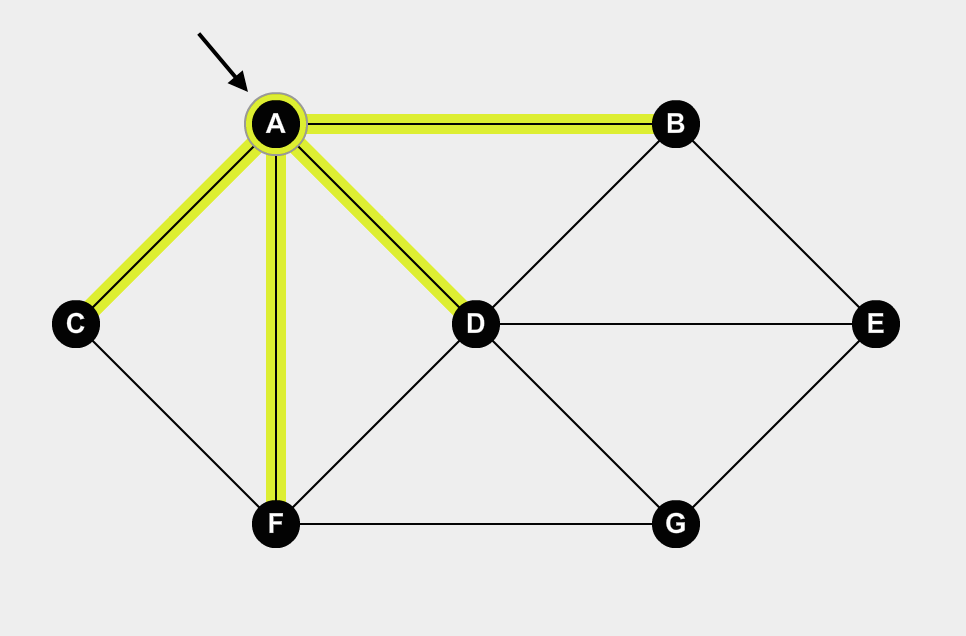
\includegraphics[width=.4\linewidth]{q3-a2}
  \captionof{figure}{$S_1 = \{A\}; S_2 = \{B, C, D, E, F, G\}$}
  \label{fig:test3}
\end{minipage}%
\begin{minipage}{.5\textwidth}
  \centering
  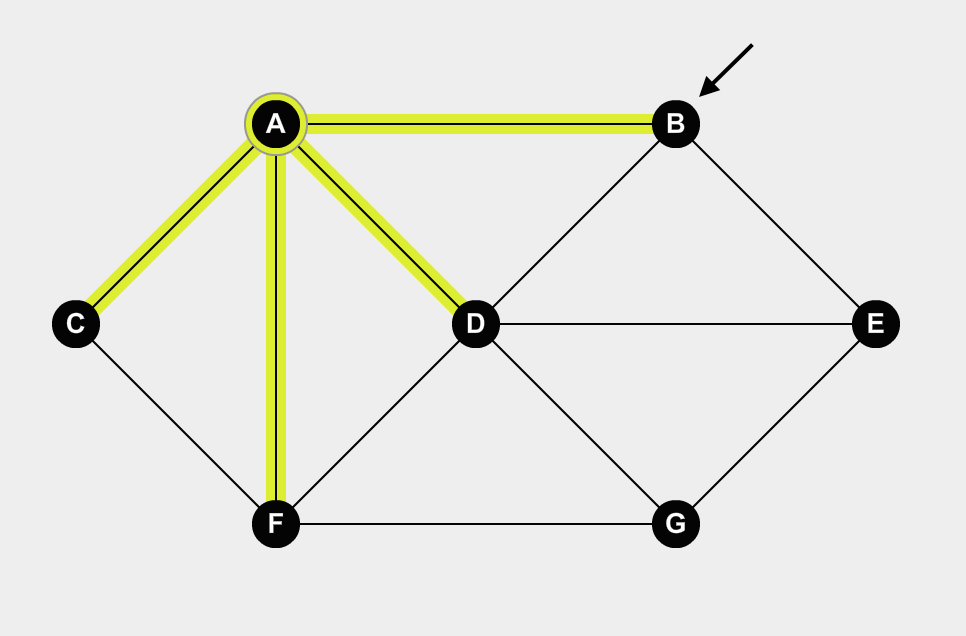
\includegraphics[width=.4\linewidth]{q3-b1}
  \captionof{figure}{Internal edges $\geq$ External edges}
  \label{fig:test4}
\end{minipage}
\end{figure}

\vspace*{3cm}

    \begin{figure}[ht]
\centering
\begin{minipage}{.5\textwidth}
  \centering
  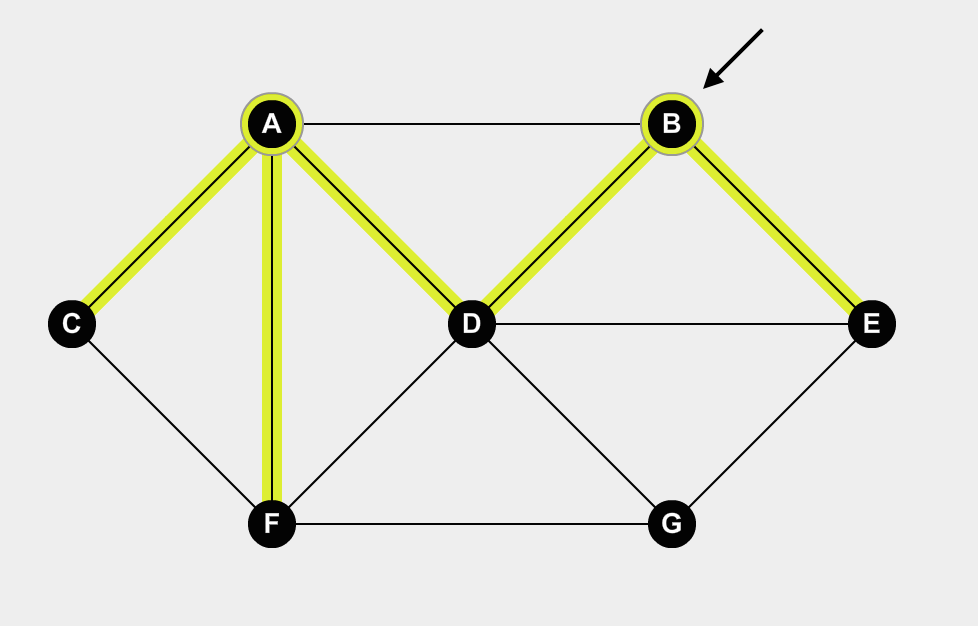
\includegraphics[width=.4\linewidth]{q3-b2}
  \captionof{figure}{$S_1 = \{A, B\}; S_2 = \{C, D, E, F, G\}$}
  \label{fig:test5}
\end{minipage}%
\begin{minipage}{.5\textwidth}
  \centering
  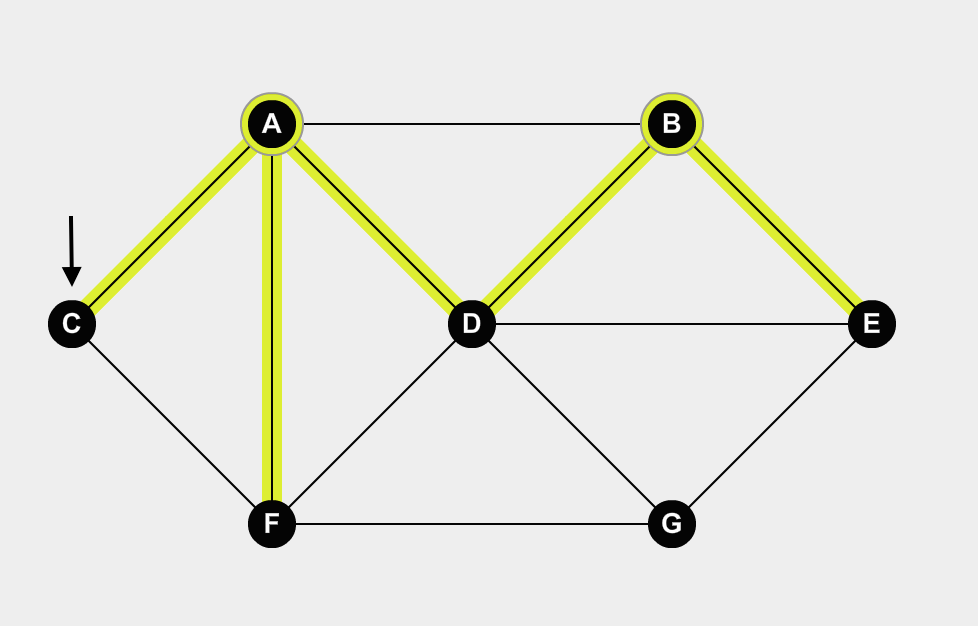
\includegraphics[width=.4\linewidth]{q3-c1}
  \captionof{figure}{Internal edges $\geq$ External edges}
  \label{fig:test6}
\end{minipage}
\end{figure}

\vspace*{3cm}

    \begin{figure}[ht]
\centering
\begin{minipage}{.5\textwidth}
  \centering
  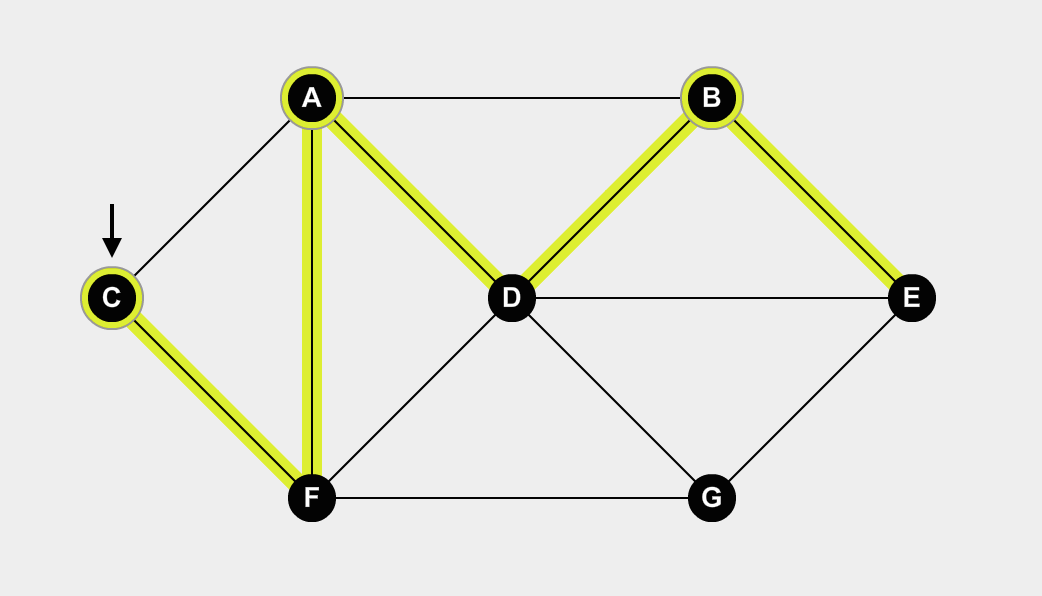
\includegraphics[width=.4\linewidth]{q3-c2}
  \captionof{figure}{$S_1 = \{A, B, C\}; S_2 = \{D, E, F, G\}$}
  \label{fig:test7}
\end{minipage}%
\begin{minipage}{.5\textwidth}
  \centering
  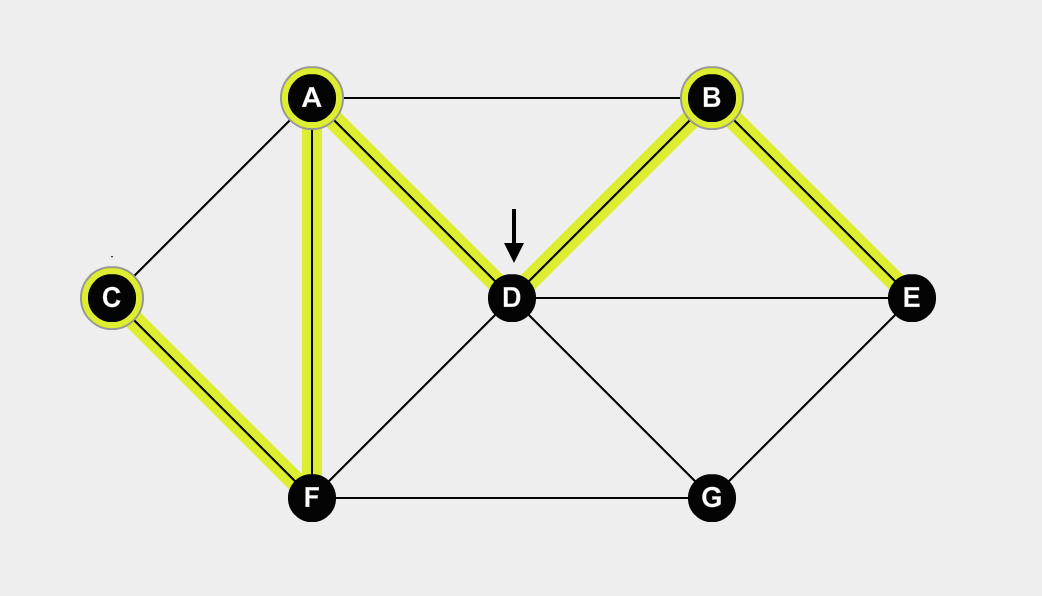
\includegraphics[width=.4\linewidth]{q3-d1}
  \captionof{figure}{Internal edges $\geq$ External edges}
  \label{fig:test8}
\end{minipage}
\end{figure}

    \begin{figure}[ht]
\centering
\begin{minipage}{.5\textwidth}
  \centering
  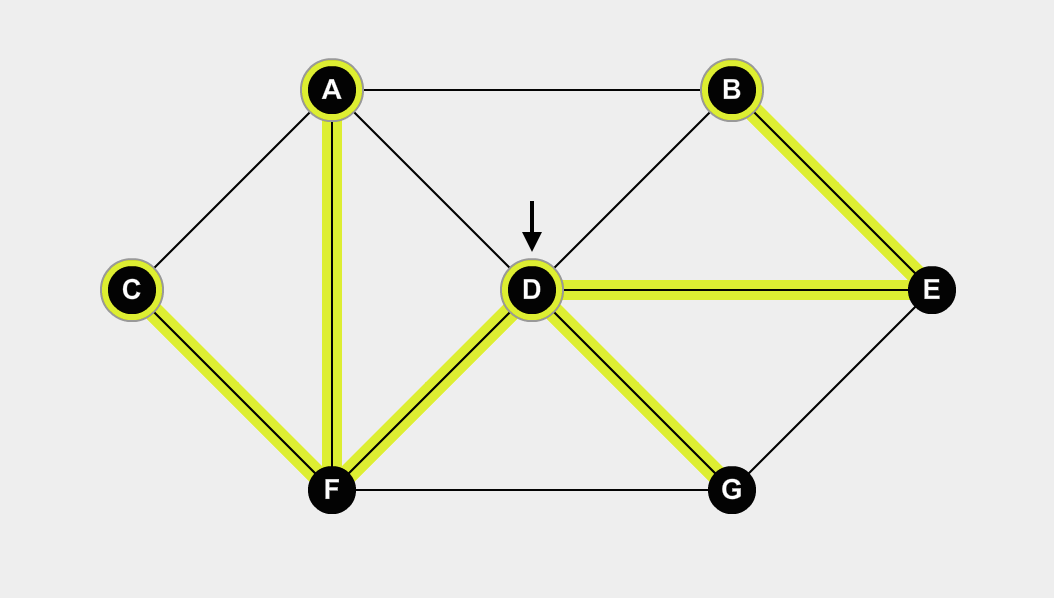
\includegraphics[width=.4\linewidth]{q3-d2}
  \captionof{figure}{$S_1 = \{A, B, C, D\}; S_2 = \{E, F, G\}$}
  \label{fig:test9}
\end{minipage}%
\begin{minipage}{.5\textwidth}
  \centering
  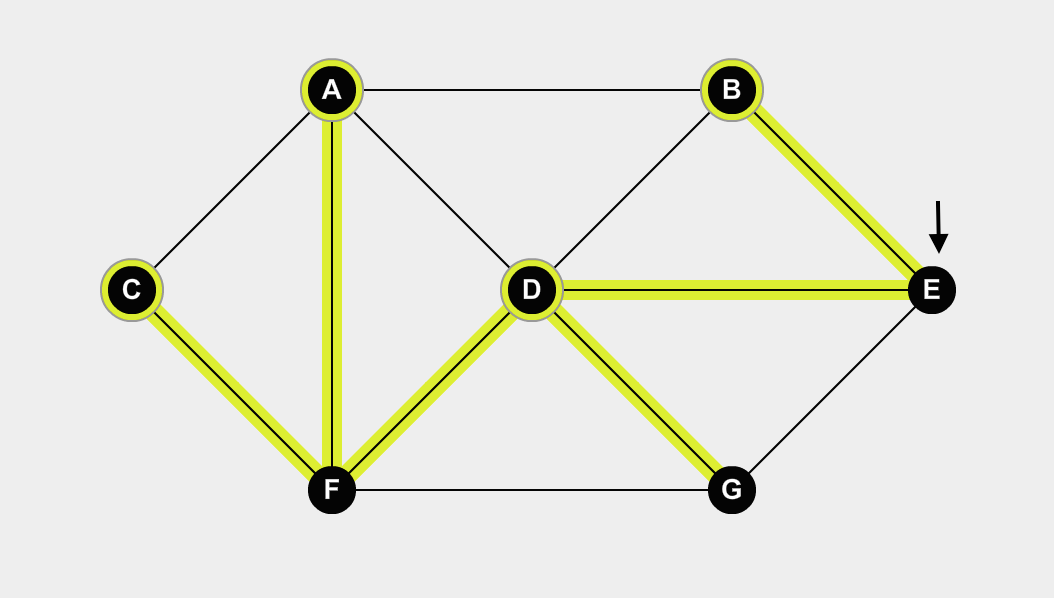
\includegraphics[width=.4\linewidth]{q3-e1}
  \captionof{figure}{Internal edges $\ngeq$ External edges}
  \label{fig:test10}
\end{minipage}
\end{figure}

    \begin{figure}[ht]
\centering
\begin{minipage}{.5\textwidth}
  \centering
  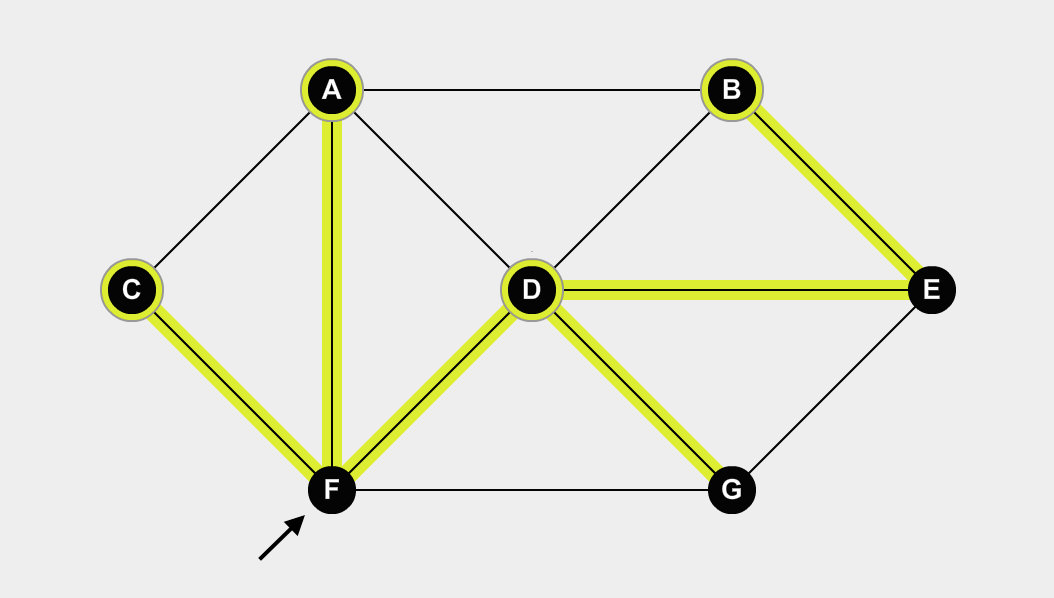
\includegraphics[width=.4\linewidth]{q3-f1}
  \captionof{figure}{Internal edges $\ngeq$ External edges}
  \label{fig:test11}
\end{minipage}%
\begin{minipage}{.5\textwidth}
  \centering
  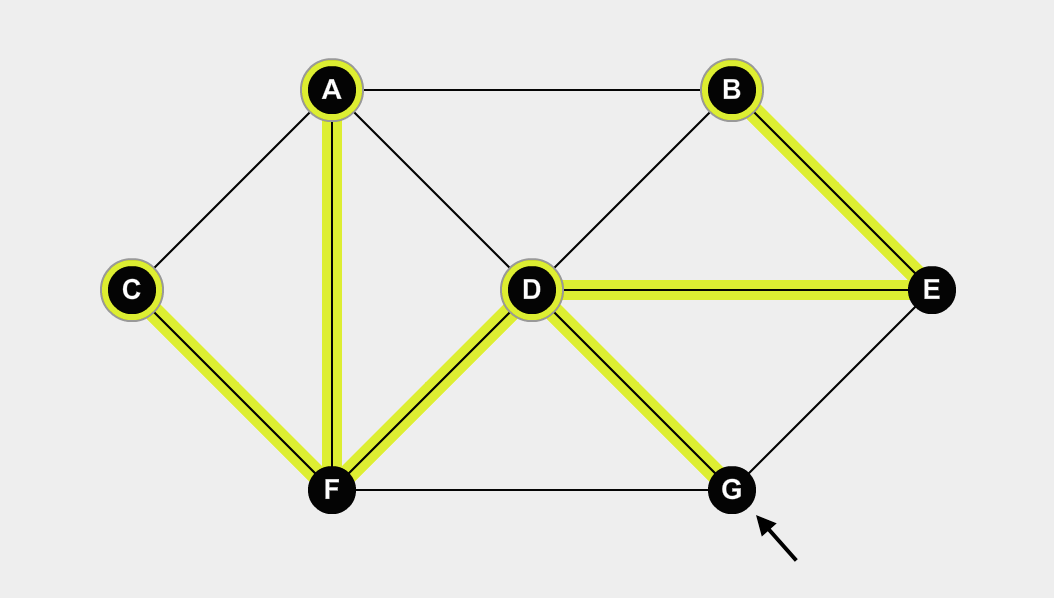
\includegraphics[width=.4\linewidth]{q3-g1}
  \captionof{figure}{Internal edges $\geq$ External edges}
  \label{fig:test12}
\end{minipage}
\end{figure}

    \begin{figure}[ht]
\centering
\begin{minipage}{.5\textwidth}
  \centering
  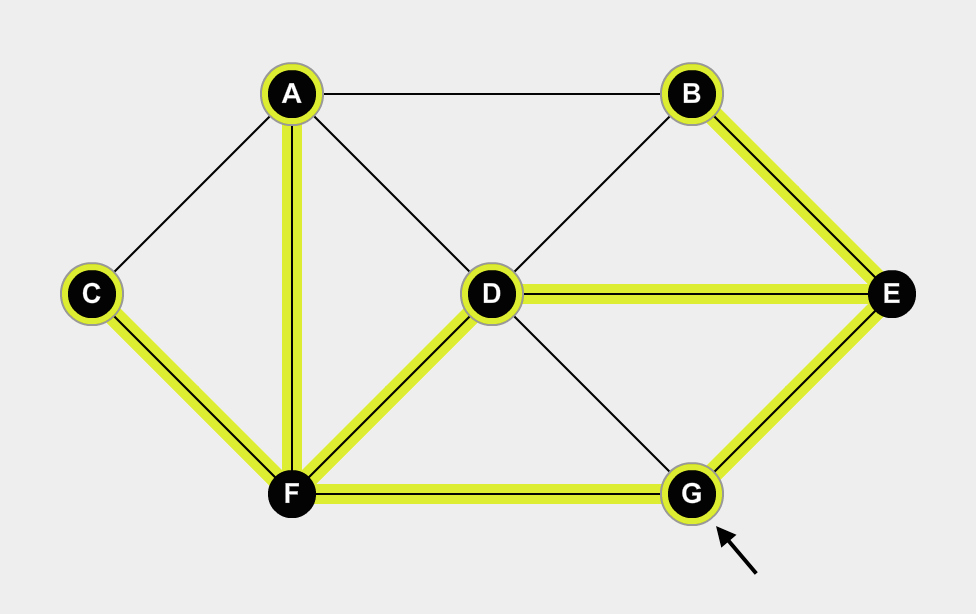
\includegraphics[width=.4\linewidth]{q3-g2}
  \captionof{figure}{$S_1 = \{A, B, C, D, G\}; S_2 = \{E, F\}$}
  \label{fig:test13}
\end{minipage}%
\begin{minipage}{.5\textwidth}
  \centering
  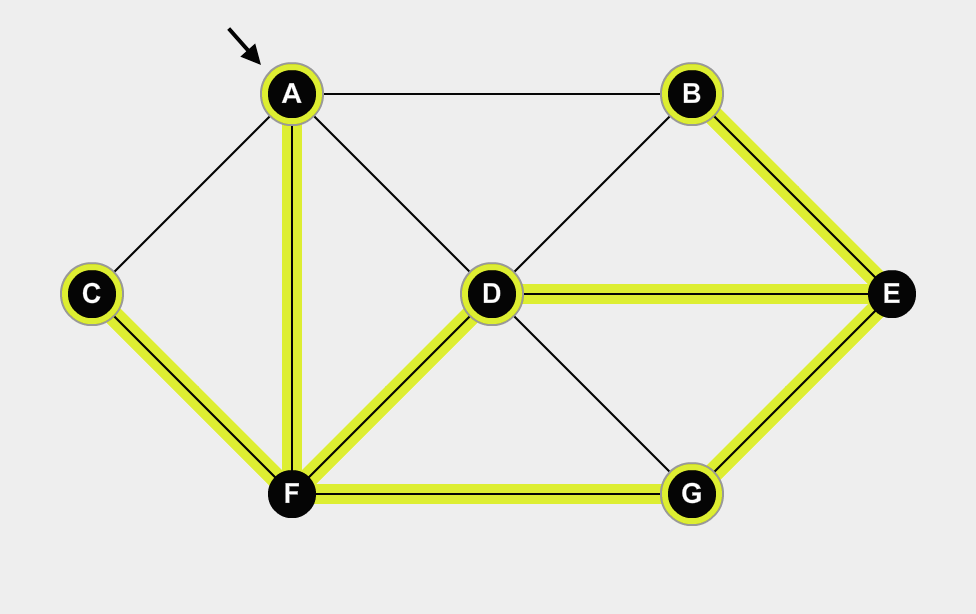
\includegraphics[width=.4\linewidth]{q3-a3}
  \captionof{figure}{Internal edges $\geq$ External edges}
  \label{fig:test14}
\end{minipage}
\end{figure}

	\begin{figure}[ht]
	\begin{center}

	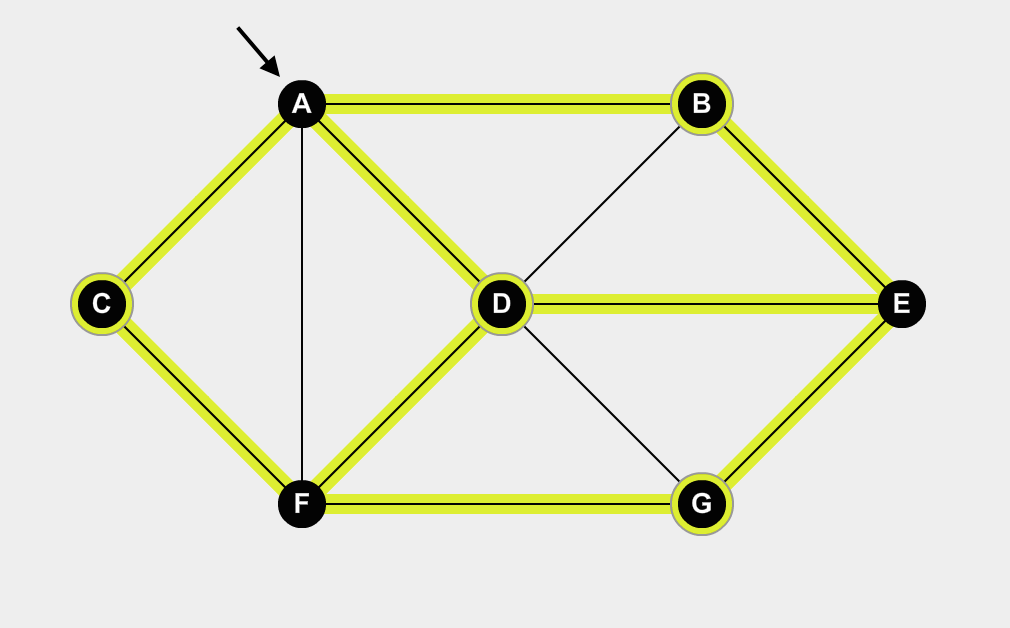
\includegraphics[scale=0.2]{q3-a4}
	\caption{$S_1 = \{B, C, D\}; S_2 = \{A, E, F\} = \proc{Max-Cut}$}

	\end{center}
	\end{figure}
    

\clearpage
    
	\item \textbf{(5 marks)}. Give a counter example to show that your greedy 
    algorithm does not always generate an optimal result.
    \par
    \textbf{Solution:}
    \par
    
    The algorithm may not produce the optimal result in the case of a bipartite graph. 
\end{enumerate}

\end{homeworkProblem}

\end{document}














 to your LaTeX file where you want your
% title page.
%
%%%%%%%%%%%%%%%%%%%%%%%%%%%%%%%%%%%%%%%%%

%-------------------------------------------------------------------------------
%	PACKAGES AND OTHER DOCUMENT CONFIGURATIONS
%-------------------------------------------------------------------------------

\documentclass{article}

\usepackage{amsmath}
\usepackage{amssymb} % Needed for certain math elements
\usepackage{clrscode3e} % Intro to Algorithms style pseudo-code
\usepackage{fancyhdr}
\usepackage{extramarks}
\usepackage{graphicx} % Required for the inclusion of images
\usepackage{enumerate}
\usepackage[parfill]{parskip} % Creates newline between paragraphs
\usepackage{rotating} % sideways table
\usepackage{caption}

% <paste>
%
% Homework Details
%   - Title
%   - Due date
%   - Class
%   - Section/Time
%   - Instructor
%   - Author
%

\newcommand{\hmwkTitle}{DAA Assignment}
\newcommand{\hmwkDueDate}{May 16, 2016}
\newcommand{\hmwkClass}{COMP3001}
\newcommand{\hmwkClassTime}{Section A}
\newcommand{\hmwkClassInstructor}{Professor Isaac Newton}
\newcommand{\hmwkAuthorName}{Chris Garland (15560955)}
%
% Basic Document Settings
%

\topmargin=-0.45in
\evensidemargin=0in
\oddsidemargin=0in
\textwidth=6.5in
\textheight=9.0in
\headsep=0.25in

\linespread{1.1}

\pagestyle{fancy}
\lhead{\hmwkAuthorName}
\chead{\hmwkClass: \hmwkTitle}
\rhead{\firstxmark}
\lfoot{\lastxmark}
\cfoot{\thepage}

\renewcommand\headrulewidth{0.4pt}
\renewcommand\footrulewidth{0.4pt}

\setlength\parindent{0pt}

%
% Create Problem Sections
%

\newcommand{\enterProblemHeader}[1]{
    \nobreak\extramarks{}{Question \arabic{#1} continued on next 
    page\ldots}\nobreak{}
    \nobreak\extramarks{Question \arabic{#1} (continued)}{Question \arabic{#1} 
    continued on next page \ldots}\nobreak{}
}

\newcommand{\exitProblemHeader}[1]{
    \nobreak\extramarks{Question \arabic{#1} (continued)}{Question \arabic{#1} 
    continued on next page\ldots}\nobreak{}
    \stepcounter{#1}
    \nobreak\extramarks{Question \arabic{#1}}{}\nobreak{}
}

\setcounter{secnumdepth}{0}
\newcounter{partCounter}
\newcounter{homeworkProblemCounter}
\setcounter{homeworkProblemCounter}{1}
\nobreak\extramarks{Question \arabic{homeworkProblemCounter}}{}\nobreak{}

%
% Homework Problem Environment
%
% This environment takes an optional argument. When given, it will adjust the
% problem counter. This is useful for when the problems given for your
% assignment aren't sequential. See the last 3 problems of this template for an
% example.
%
\newenvironment{homeworkProblem}[1][-1]{
    \ifnum#1>0
        \setcounter{homeworkProblemCounter}{#1}
    \fi
    \section{Question \arabic{homeworkProblemCounter}}
    \setcounter{partCounter}{1}
    \enterProblemHeader{homeworkProblemCounter}
}{
    \exitProblemHeader{homeworkProblemCounter}
}

% </paste>
\begin{document}
\setlength{\belowdisplayskip}{1.2cm}
\setlength{\belowdisplayshortskip}{1.0cm}

\begin{titlepage}

% Defines a new command for the horizontal lines, change thickness here
\newcommand{\HRule}{\rule{\linewidth}{0.5mm}} 


\center % Center everything on the page
 
%-------------------------------------------------------------------------------
%	HEADING SECTIONS
%-------------------------------------------------------------------------------
%
\includegraphics[scale=0.3]{Curtin1}\\[1.5cm]
\textsc{\LARGE Curtin University}\\[1.5cm] % Name of your university/college
\textsc{\Large Department of Computing}\\[0.5cm] % Major heading/course name
\textsc{\large COMP3001}\\[0.5cm] % Minor heading such as course title

%-------------------------------------------------------------------------------
%	TITLE SECTION
%-------------------------------------------------------------------------------

\HRule \\[0.4cm]
{ \huge \bfseries Design and Analysis of Algorithms Assignment}\\[0.4cm] % Title
\HRule \\[1.5cm]
 
%-------------------------------------------------------------------------------
%	AUTHOR SECTION
%-------------------------------------------------------------------------------

\begin{minipage}{0.4\textwidth}
\begin{flushleft} \large
\emph{Author: 15560955}\\
Chris \textsc{Garland} % Your name
\end{flushleft}
\end{minipage}
~
\begin{minipage}{0.4\textwidth}
\begin{flushright} \large
\emph{Lecturer:} \\
Dr. Sie Teng \textsc{Soh} % Supervisor's Name
\end{flushright}
\end{minipage}\\[4cm]

% If you don't want a supervisor, uncomment the two lines below and remove the section above
%\Large \emph{Author:}\\
%John \textsc{Smith}\\[3cm] % Your name

%-------------------------------------------------------------------------------
%	DATE SECTION
%-------------------------------------------------------------------------------

{\large \today}\\[3cm] % Date, change the \today to a set date if you want to be precise

%-------------------------------------------------------------------------------
%	LOGO SECTION
%-------------------------------------------------------------------------------

% Include a department/university logo - this will require the graphicx package

\includegraphics[scale=0.25]{Curtin2}
 
%-------------------------------------------------------------------------------

\vfill % Fill the rest of the page with whitespace

\end{titlepage}

%-------------------------------------------------------------------------------
% Question 1
%-------------------------------------------------------------------------------
\begin{homeworkProblem}
\begin{enumerate}[a)]
	\item \textbf{(10 marks).} Use the Master method to solve the following 
    recurrence function:
    	\begin{equation}
			T(n) = 3T(\sqrt[2]{n}) + \log_2 n
		\end{equation}
	\textbf{Solution:}
    \par
    Given the master theorem:
    \begin{equation}
		T(n) = aT(n/b) + f(n)
	\end{equation}
    \par 
    We can see that $a = 3$, $b = \sqrt{n}$ and $f(n) = \log_2 n$. As $b$ does not 
    conform to the master theorem, we will use a change of variable:
    \par 
    
    \textit{let}: $n = 2^{m} \therefore \log_2 n = m$ \\
    $\hspace*{1.87cm} \therefore \sqrt[2]{n} = 2^{m/2}$
    \begin{equation}
		T(2^{m}) = 3T(2^{m/2}) + m
	\end{equation}
    \par 
    Now, we perform another substitution \ldots
    \par
    \textit{let}: $T(2^{m}) = S(m)$\\
    \textit{let}: $T(2^{m/2}) = S(m/2)$
    \begin{equation}
		S(m) = 3S(m/2) + m
	\end{equation}
    \par 
    We now have a recurrence equation that conforms to the format of the Master 
    Theorem \ldots $a = 3$, $b = 2$ and $f(m) = m$. Lets compare $m^{\log_b a}$ with 
    $f(m)$ \ldots
    \par 
    $m^{\log_b a} = m^{\log_2 3} > f(m)$\\
    $f(m) = O(m^{\log_2 3 - \epsilon})$, where $\epsilon > 0$
    \par 
    By case 1 of Master Theorem:
    \begin{equation}
		S(m) = \Theta(m^{\log_2 3})
	\end{equation}
    We know that $S(m) = T(2^m)$ and $2^m = n \therefore$
    \begin{equation}
		T(n) = \Theta(m^{\log_2 3})
	\end{equation}
    Given that $m = \log_2 n$ \ldots
    \begin{equation}
    \begin{aligned}
		T(n) &= \Theta((\log_2 n)^{\log_2 3})\\
        &= \Theta(\log_2^{\log_2 3} n)
	\end{aligned}
	\end{equation}
    
    
\end{enumerate}
\end{homeworkProblem}

\clearpage

%-------------------------------------------------------------------------------
% Question 2
%-------------------------------------------------------------------------------
\begin{homeworkProblem}
Consider the following communication network that is represented by a weighted 
graph $G = (V, E)$ in which the non-negative number $r_{u,v}$ represents the 
\textit{operational probability} or \textit{reliability} of link 
$(u, v) \in E$ for $0 \leq r_{u,v} \leq 1.0$. Recall that a path $P_{a,b}$ is a 
sequence of links from a given source node $a$ to its destination node $b$. The 
reliability of a path (called \textit{path reliability}), $r_{a,b}$, is computed 
by multiplying the reliability of each link in path $P_{a,b}$. For example of 
path $P_{A,E} =$ (A, D, B, E) from source node A to destination node E is 
$R_{A,E} = (0.9 * 0.85 * 0.8) = 0.612$. We define \textit{the most reliable path} 
from a source node $s$ to a destination node $t$ as the path with the highest 
reliability among all possible paths form $s$ to $t$, i.e., the maximum 
$R_{s,t}$. \\[2cm]

\begin{figure}[h]
\begin{center}

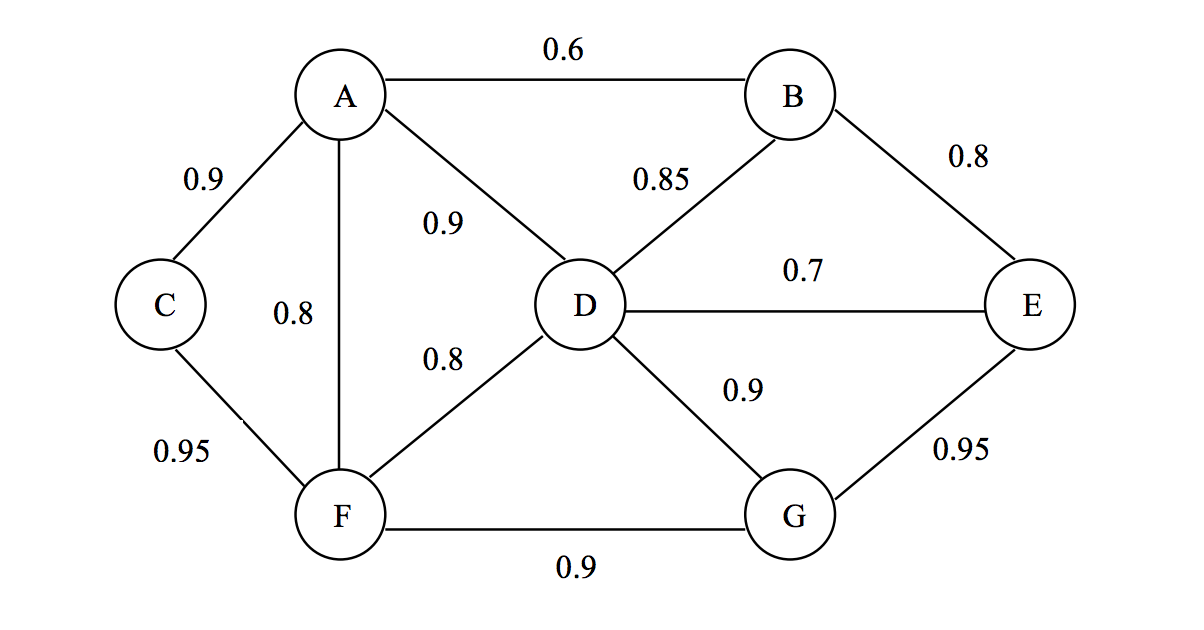
\includegraphics[scale=0.77]{Diag1}
\caption{Weighted graph representation of a communication network}

\end{center}
\end{figure}

\clearpage

\begin{enumerate}[a)]
	\item \textbf{(25 marks).} Design a \textit{greedy} algorithm that generates 
    the most reliable path from a source node $s$ to every destination node $t$ 
    in the network. 
    \par
	\textbf{Solution:}
    \par

    In this design we will modify Dijkstra's algorithm to \textit{greedily} 
    determine the most reliable path from a source node $s$ to every destination 
    node in the network. Original time complexity is maintained: 
    $O(|E| + |V|\log_2|V|)$ \ldots
    
    \begin{codebox}
    \Procname{$\proc{Dijkstra-Modified}(G, w, s)$}
    \li $\proc{Initialize-Single-Source}(G,s)$
    \li $S = \emptyset$
    \li $Q = \attribxx{G}{V}$
    \li \While $Q \neq \emptyset$
   	\li 	\Do
    		    $u = \proc{Extract-Max}(Q)$\>\>\>\>\>\>\Comment Modification
                \textit{from}: $u =$ \proc{Extract-Min}(Q)
    \li         $S = S\ \cup\ \{u\}$
    \li 	    \For each vertex $v \in \attrib{G}{Adj[u]}$
    \li             \Do
                        $\proc{Relax(u, v, w)}$
                    \End
            \End        
    \end{codebox}
    
    Line 1 initializes the $d$ and $\pi$ values as shown below. Line 2 initializes 
    the set $S$ to the empty set. Line 3 initializes the \textit{max-priority} 
    queue $Q$ to contain all the vertices in $V$. Each time through the 
    \textbf{while} loop of lines 4--8, line 5 extracts a vertex from $Q$ and line 
    6 adds it to $S$. Lines 7--8 relax each edge $(u, v)$ and updates the estimate 
    \attrib{v}{d} if the path reliability can be improved.
    
    \begin{codebox}
    \Procname{$\proc{Initialize-Single-Source}(G, s)$}
    \li \For each vertex $v \in \attribxx{G}{V}$
   	\li     \Do
    			$\attribxx{v}{d} = 0$\>\>\>\>\>\>\Comment Modification 
                \textit{from}: \attrib{v}{d} $= \infty$
    \li         $\attribxx{v}{\pi} = \const{nil}$\>\>\>\>\>\>\Comment $v$'s 
    												predecessor
            \End
    \li $\attribxx{s}{d} = 1$\>\>\>\>\>\>\>\Comment Modification \textit{from}: 
    \attrib{s}{d} $= 0$
    \end{codebox}
    
    We modify by initializing the \textit{reliability} attribute 
    $\attribxx{v}{d}$, of all $v \in V - \{s\}$ to $0$, which is a lower bound 
    on the weight/reliability of a path from source $s$ to $v$. We call 
    $\attribxx{v}{d}$ a path reliability estimate. The path-reliability attribute 
    $\attribxx{s}{d}$ of the source node $s$ is initialized to $1$ 
    (max reliability). 
    
    \begin{codebox}
    \Procname{$\proc{Relax}(u, v, w)$}
    \li \If $\attrib{v}{d} < \attrib{u}{d} \times w(u, v)$\>\>\>\>\>\>\>\Comment 
    		Modification \textit{from}: $\attrib{v}{d} > \attrib{u}{d} + w(u, v)$
    \li 	\Do
    			$\attrib{v}{d} = \attrib{u}{d} \times w(v, v)$\>\>\>\>\>\>\Comment
                Modification \textit{from}: $\attrib{v}{d} = \attrib{u}{d} +
                w(u, v)$
    \li 		$\attrib{v}{\pi} = u$\>\>\>\>\>\>\Comment $v$'s predecessor
    		\End
    \end{codebox}
    
    \begin{figure}[h]
		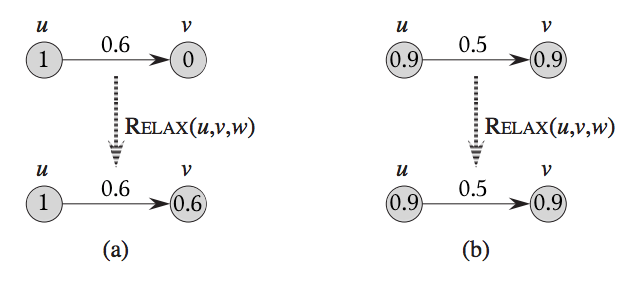
\includegraphics[scale=0.8]{Relax}
        \caption[caption]{\textbf{(a)} Because the value of $\attrib{v}{d} < 
        		 \attrib{u}{d} \times w(u, v)$ prior to relaxation, the value of 
                 \attrib{v}{d} is updated. 
                 \\\hspace*{1.53cm}\textbf{(b)} Here, $\attrib{v}{d} \geq 
                 \attrib{u}{d} \times w(u, v)$ before relaxation, and so 
                 \attrib{v}{d} remains unchanged. }
	\end{figure}
    
    \clearpage
    
    \item \textbf{(15 marks)}. Use your algorithm in part a) to generate the most 
    reliable path from node A to every other node in the given graph. List the 
    most reliable paths and their corresponding path reliabilities.
    \par
    \textbf{Solution:}
    \par
    \vspace*{7cm}
    \begin{center}
    \textit{On Next Page \ldots}
	\end{center}
%==============================================================================
\begin{sidewaystable}[ht]
\centering
\resizebox{\columnwidth}{!}{%
%\caption{My caption}
\label{my-label}
\begin{tabular}{ccccccccccc}
\textbf{Step \#} & \textbf{Unvisited($Q$)} & \textbf{Visited($S$)} & \textbf{Current($u$)} & \multicolumn{7}{l}{\textbf{Reliability of Path to Vertex($v$): (reliability{[}$s$-$v${]}, predecessor($\pi$))$_{iteration}$}} \\
\multicolumn{1}{l}{}                 & \multicolumn{1}{l}{}                      & \multicolumn{1}{l}{}                    & \multicolumn{1}{l}{}                    & \textbf{A($s$)}  & \textbf{B}   & \textbf{C}  & \textbf{D}  & \textbf{E}    & \textbf{F}   & \textbf{G}  \\
\textbf{Init}                        & \{A, B, C, D, E, F, G\}                   & \{-\}                                   & N/A                                     & (1, -)$_0$        & (0, -)$_0$    & (0, -)$_0$   & (0, -)$_0$   & (0, -)$_0$     & (0, -)$_0$    & (0, -)$_0$   \\
\textbf{1}                           & \{B, C, D, E, F, G\}                      & \{A\}                                   & A                                       & (1, -)$_0$        & (0.6, A)$_1$    & (0.9, A)$_1$   & (0.9, A)$_1$   & (0, -)$_0$     & (0.8, A)$_1$    & (0, -)$_0$   \\
\textbf{2}                           & \{B, D, E, F, G\}                         & \{A, C\}                                & C                                       & (1, -)$_2$        & (0.6, A)$_1$    & (0.9, A)$_1$   & (0.9, A)$_1$   & (0, -)$_0$     & (0.855, C)$_2$  & (0, -)$_0$   \\
\textbf{3}                           & \{B, E, F, G\}                            & \{A, C, D\}                             & D                                       & (1, -)$_3$        & (0.765, D)$_3$  & (0.9, A)$_1$   & (0.9, A)$_1$   & (0.63, D)$_3$    & (0.855, C)$_3$  & (0.81, D)$_3$  \\
\textbf{4}                           & \{B, E, G\}                               & \{A, C, D, F\}                          & F                                       & (1, -)$_4$        & (0.765, D)$_3$  & (0.9, A)$_4$   & (0.9, A)$_4$   & (0.63, D)$_3$    & (0.855, C)$_3$  & (0.81, D)$_3$  \\
\textbf{5}                           & \{B, E\}                                  & \{A, C, D, F, G\}                       & G                                       & (1, -)$_4$        & (0.765, D)$_3$  & (0.9, A)$_4$   & (0.9, A)$_5$   & (0.7695, G)$_5$  & (0.855, C)$_5$  & (0.81, D)$_3$  \\
\textbf{6}                           & \{B\}                                     & \{A, C, D, E, F, G\}                    & E                                       & (1, -)$_4$        & (0.765, D)$_6$  & (0.9, A)$_4$   & (0.9, A)$_6$   & (0.7695, G)$_5$  & (0.855, C)$_5$  & (0.81, D)$_6$  \\
\textbf{7}                           & \{-\}                                     & \{A, B, C, D, E, F, G\}                 & B                                       & (1, -)$_7$        & (0.765, D)$_6$  & (0.9, A)$_4$   & (0.9, A)$_7$   & (0.7695, G)$_7$  & (0.855, C)$_5$  & (0.81, D)$_6$ 
\end{tabular}
}%
\end{sidewaystable}
%===============================================================================
\end{enumerate}
\end{homeworkProblem}

\clearpage

%-------------------------------------------------------------------------------
% Question 3
%-------------------------------------------------------------------------------
\begin{homeworkProblem}
Consider an undirected graph $G = (V, E)$, where $V$ is a set of nodes and $E$ 
is a  set of links. As an example, consider the following graph, where each 
link is  labeled by a lower case letter, e.g., link $a$ connects nodes A and C. 
As defined  in Chapter 23 of the textbook (Introduction to Algorithms by Cormen, 
et al), a  cut $(S, V – S)$ is a partition of nodes in $V$. Further, a link 
$(u, v) \in E$ \textit{crosses} the cut $(S, V – S)$ if \textbf{either} node 
$u \in S$ and $v \in (V – S)$ \textbf{or} node $u \in (V – S)$ and  $v \in S$; 
i.e., one of its end points is in $S$ and the other is in  $V – S$. As an  
example, $S_1 = \{C\}$ and $S_2 = V - S_1 =$ {A, B, D, E, F, G} is a cut. 
The weight of a  cut is defined as the number of links \textbf{crossing} the cut. 
As an  example, the  weight of the cut $(S_1, S_2)$ is two; there are two 
crossing links in the cut. The \textbf{maximum cut} (called \textbf{Max-Cut}) is 
a cut with the \textbf{maximum weight}. The problem of finding a maximum cut in 
a graph is known as the \textbf{Max-Cut Problem}, a well known NP-complete 
problem. \\[2cm]

\begin{figure}[h]
\begin{center}

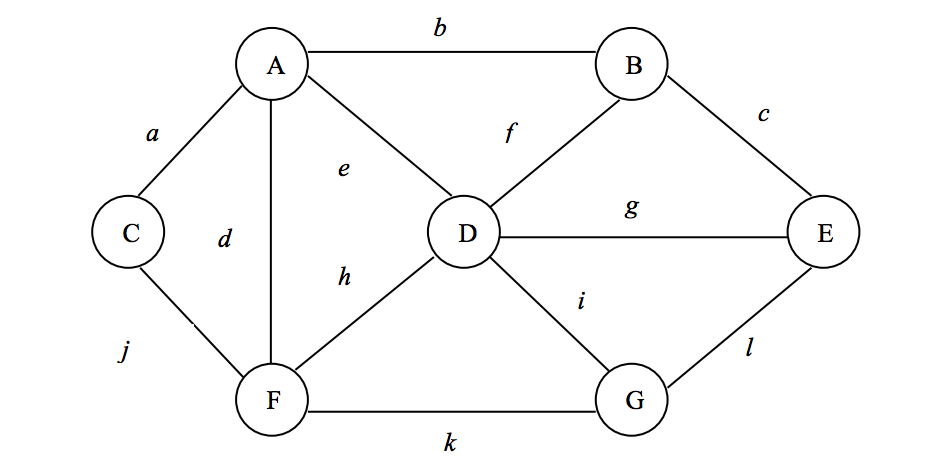
\includegraphics[scale=0.97]{Diag2}
\caption{Weighted graph representation of a communication network}

\end{center}
\end{figure}

\clearpage

\begin{enumerate}[a)]
	\item \textbf{(5 marks).} Generate all possible cuts in the given graph, and 
    determine its maximum cut.
    \par
	\textbf{Solution:}
    \par

	In order to determine the number of all possible cuts, we will use the formula \ldots 
    \begin{equation}
		2^n - 2
	\end{equation}
    Here we have $n$ as the number of vertices. This will give us the number of 
    \textit{all} possible combinations including the empty \textit{and} full sets. This is
    why we subtract $2$. This will give us the answer \ldots 
    
    \begin{equation}
    \begin{aligned}
		2^n - 2 &= 2^7 - 2\\
        &= 126
	\end{aligned}
	\end{equation}
    
    This is the number of all possible cuts. \\
    \par
    In the figure below will provide the \proc{Max-Cut} \ldots
    
    \vspace*{3cm}
    
	\begin{figure}[h]
	\begin{center}

	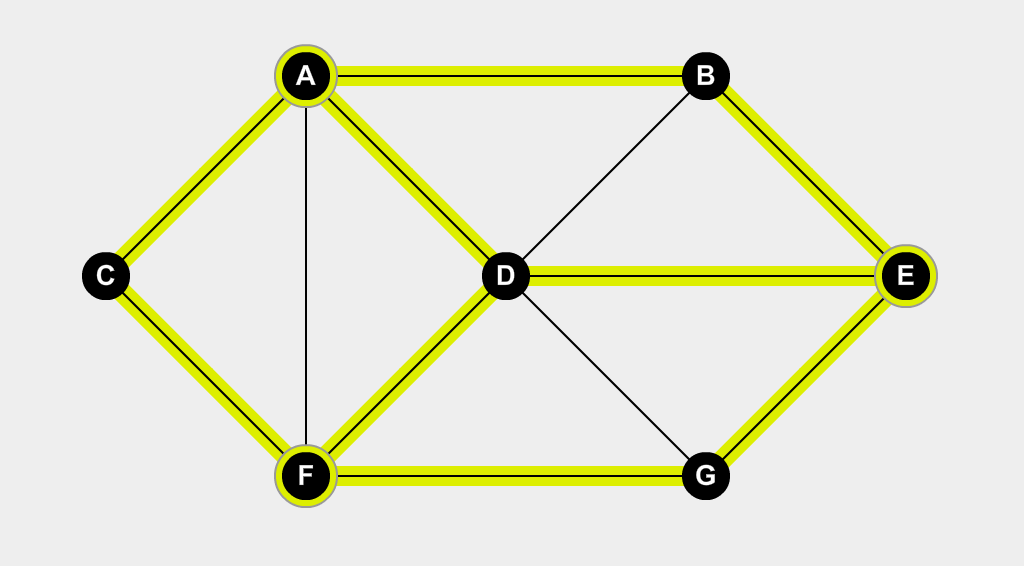
\includegraphics[scale=0.5]{max-cut}
	\caption{Max-Cut of graph illustrated in previous figure}

	\end{center}
	\end{figure}
    
    \clearpage

    \item \textbf{(20 marks)}. Design a \textit{greedy} algorithm to solve the 
    Max-Cut problem. As part of your solution, you must state your \textit{greedy 
    criteria}. Further, show your algorithm in a concise but clear pseudo-code. 
    You must explain in detail each line of the pseudo-code and show how to 
    implement the algorithm so that it has the best possible time complexity.
    \par
    \textbf{Solution:}
    \par
    
    In this design we follow the greedy approach of making the locally optimal choice at 
    each stage with the hope of finding a global optimum. the idea behind this algorithm
    is that we have two sets $S_1$ and $S_2$. $S_1$ will be initialized to contain the
    first vertex $v \in \attrib{G}{V}$ (A in this case). $S_2$ will be initialized to 
    $\attrib{G}{V} - S_1$ (all other vertices). Now we have $(S_1 = \{A\}, S_2 = 
    \{B, C, D, E, F, G\})$. Lets consider vertex A $\in S_1$. The number of cuts is
    determined by the number of adjacent vertices in $S_2$. In this case we have 4, 
    $\{B, C, D, F\}$. We will call this set \textit{external vertices}. Any vertices in 
    the same set, we will call \textit{internal vertices}. The algorithm runs through each 
    $v \in \attrib{G}{V}$ and determines whether the number of \textit{internal vertices}
    $\geq$ the number of \textit{external vertices} \textbf{\textit{(greedy criteria)}}. 
    If so, then swap sets and maintain a boolean value to be use as a loop terminator.
    Once there is no more improvement, we have our final cut.\\
    \par 
    \textbf{Input:} Graph (all vertices \attrib{G}{V}, adjacency list \attrib{G}{adj[u]})
    \\
    \textbf{Output:} \proc{Max-Cut}  

	\begin{codebox}
    \Procname{$\proc{Max-Cut}(G)$}
    \li $S_1 = 1st \in \attrib{G}{V}$
    \li $S_2 = \attribxx{G}{V} - S_1$
    \li \textbf{do} 
   	\li 	\Do
    		    improvement = \const{false}
    \li 	    \For each vertex $u \in \attrib{G}{V}$
    \li             \Do
                        \If (num $v \in \attrib{G}{adj[u]}$) $\in$ current set 
                        $\geq$\\ 
                        \hspace*{1.92cm}(num $v \in \attrib{G}{adj[u]}$) $\in$ 
                        other set
	\li						\Do
    							\proc{Swap-Sets$(u, S_1, S_2)$}
    \li                         improvement = \const{true}
    						\End
                    \End
            \End 
    \li \While improvement
    \li \Return $(S_1, S_2)$
    \end{codebox}
    
    Lines 1--2 initialize the sets. In this case, to $(\{A\}, \{B, C, D, E, F, G\})$. The
    \textbf{do} - \While loop on lines 3--9 will terminate if the boolean value on Line 4 
    is not adjusted to \const{true}. The \For loop on lines 5--8 will iterate over every 
    vertex $v \in \attrib{G}{V}$. The \If statement on line 6 is what makes this algorithm 
    greedy. \If number of \textit{internal vertices} $\geq$ number \textit{external 
    vertices} then swap sets and maintain bool value to keep the loop going. Finally when 
    there does not exist a vertex that has a greater number of \textit{internal vertices}, 
    Line 10 will \Return the max-cut. 
    
    \begin{codebox}
	\Procname{$\proc{Swap-Sets}(u)$}
    \li \If $\attrib{u}{currentSet} \isequal S_1$
    \li 	\Do 
    			$S_1 = S_1 - \{u\}$
    \li         $S_2 = S_2 \cup \{u\}$
    \li 		$\attrib{u}{currentSet} = S_2$
    		\End 
    \li \Else
    \li		\Do 
            	$S_2 = S_2 - \{u\}$
    \li         $S_1 = S_1 \cup \{u\}$
    \li 		$\attrib{u}{currentNode} = S_1$
    		\End 
	\end{codebox}

	\clearpage

    \item \textbf{(10 marks)}. Use your algorithm in part b) to generate the 
    Max-Cut of the given graph. Does your algorithm generate an optimal result? 
    \par
    \textbf{Solution:}
    \par 
	\vspace*{7cm}
    
    \begin{center}
    \textit{On Next Page} \ldots
	\end{center}

    \clearpage
        
  \vspace*{2cm}
  
    \begin{figure}[ht]
\centering
\begin{minipage}{.5\textwidth}
  \centering
  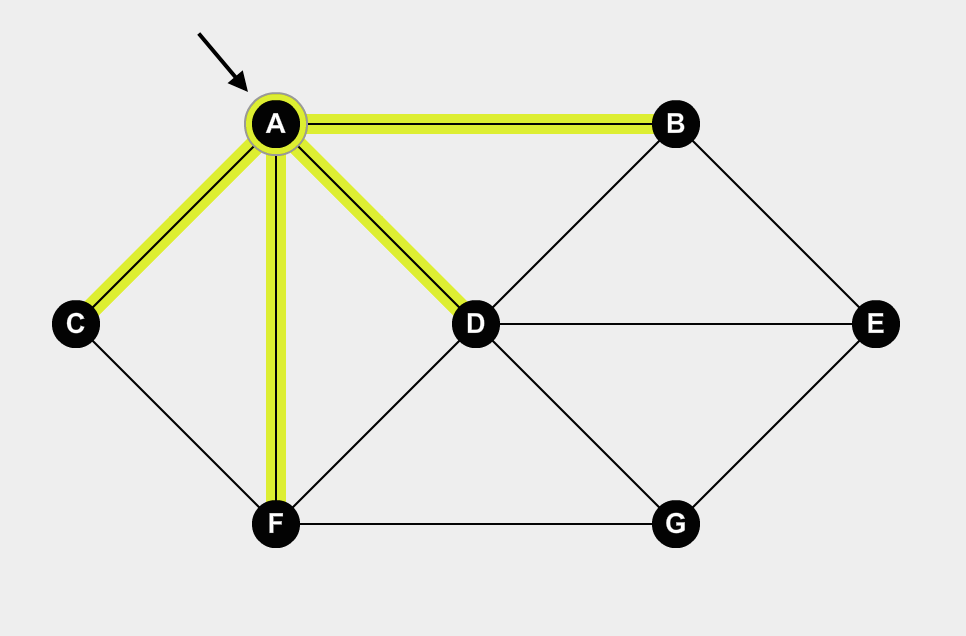
\includegraphics[width=.4\linewidth]{q3-a2}
  \captionof{figure}{$S_1 = \{A\}; S_2 = \{B, C, D, E, F, G\}$}
  \label{fig:test3}
\end{minipage}%
\begin{minipage}{.5\textwidth}
  \centering
  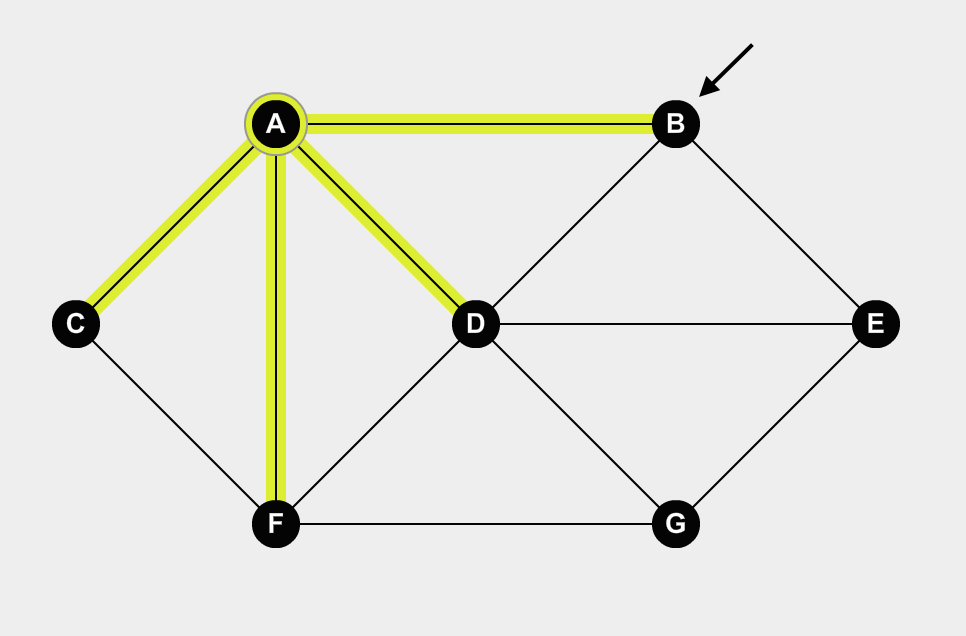
\includegraphics[width=.4\linewidth]{q3-b1}
  \captionof{figure}{Internal edges $\geq$ External edges}
  \label{fig:test4}
\end{minipage}
\end{figure}

\vspace*{3cm}

    \begin{figure}[ht]
\centering
\begin{minipage}{.5\textwidth}
  \centering
  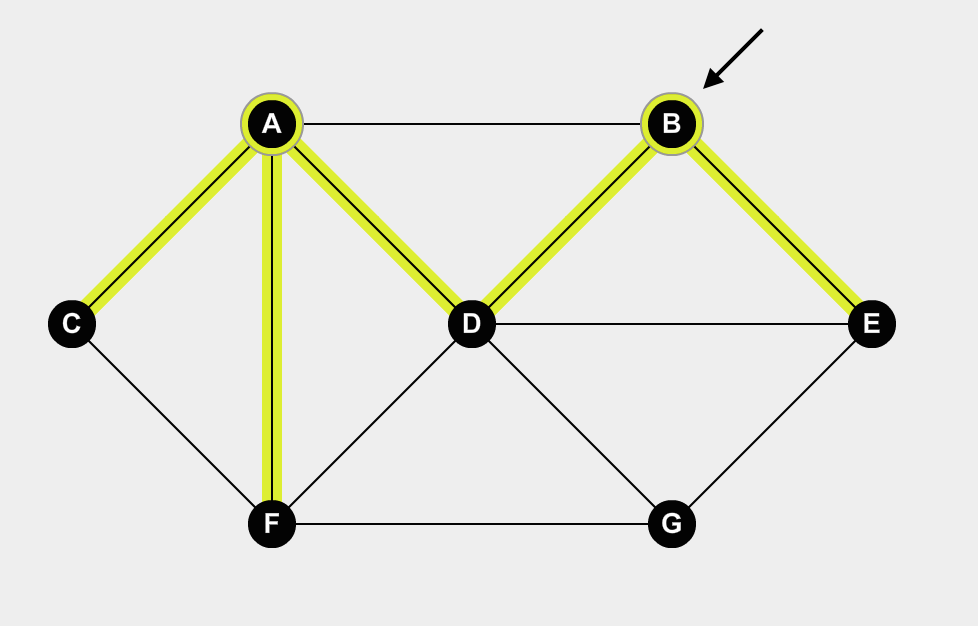
\includegraphics[width=.4\linewidth]{q3-b2}
  \captionof{figure}{$S_1 = \{A, B\}; S_2 = \{C, D, E, F, G\}$}
  \label{fig:test5}
\end{minipage}%
\begin{minipage}{.5\textwidth}
  \centering
  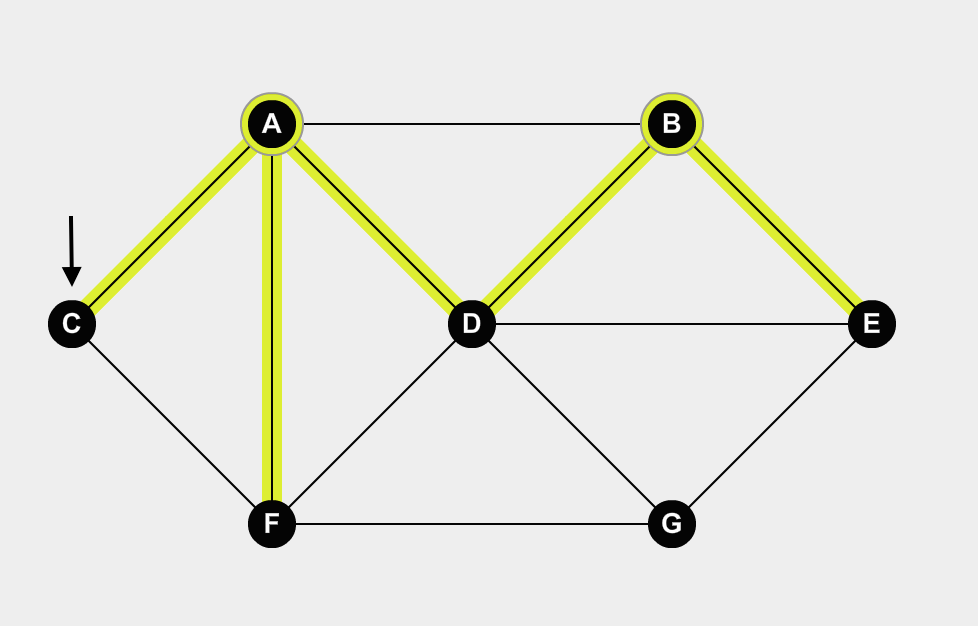
\includegraphics[width=.4\linewidth]{q3-c1}
  \captionof{figure}{Internal edges $\geq$ External edges}
  \label{fig:test6}
\end{minipage}
\end{figure}

\vspace*{3cm}

    \begin{figure}[ht]
\centering
\begin{minipage}{.5\textwidth}
  \centering
  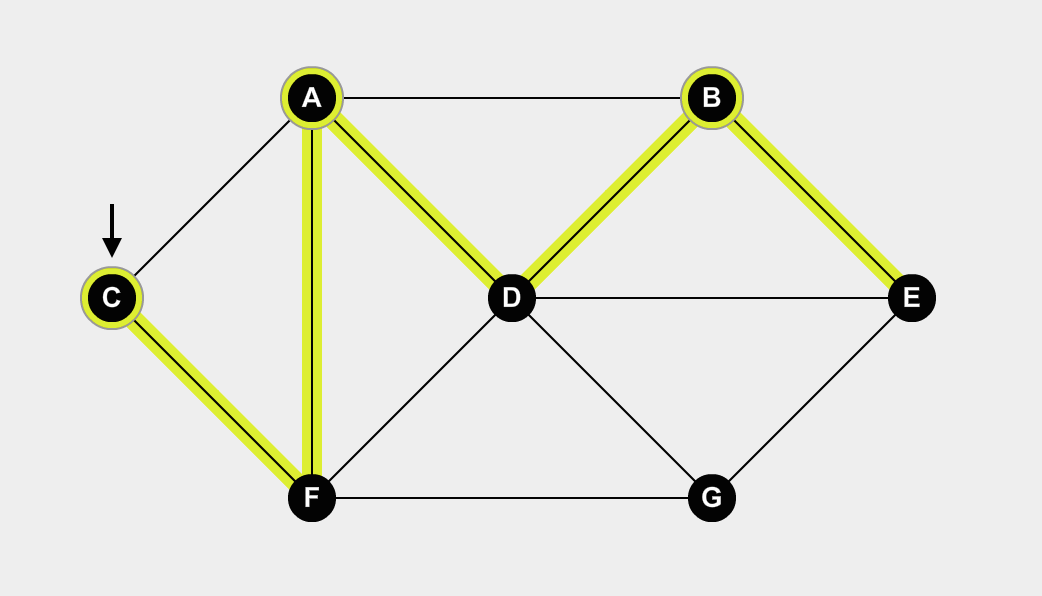
\includegraphics[width=.4\linewidth]{q3-c2}
  \captionof{figure}{$S_1 = \{A, B, C\}; S_2 = \{D, E, F, G\}$}
  \label{fig:test7}
\end{minipage}%
\begin{minipage}{.5\textwidth}
  \centering
  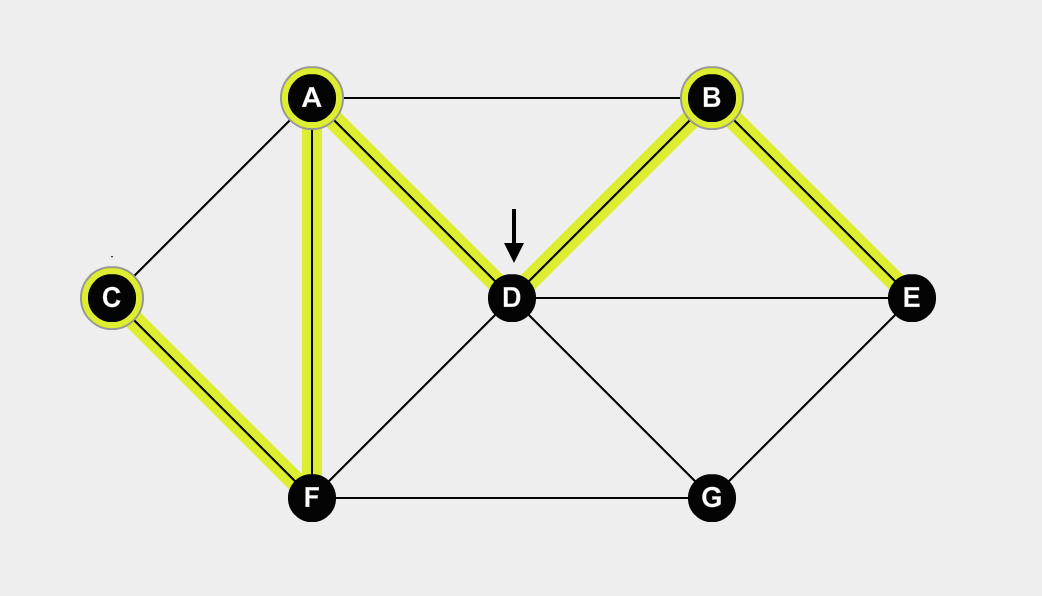
\includegraphics[width=.4\linewidth]{q3-d1}
  \captionof{figure}{Internal edges $\geq$ External edges}
  \label{fig:test8}
\end{minipage}
\end{figure}

    \begin{figure}[ht]
\centering
\begin{minipage}{.5\textwidth}
  \centering
  \includegraphics[width=.4\linewidth]{q3-d2}
  \captionof{figure}{$S_1 = \{A, B, C, D\}; S_2 = \{E, F, G\}$}
  \label{fig:test9}
\end{minipage}%
\begin{minipage}{.5\textwidth}
  \centering
  \includegraphics[width=.4\linewidth]{q3-e1}
  \captionof{figure}{Internal edges $\ngeq$ External edges}
  \label{fig:test10}
\end{minipage}
\end{figure}

    \begin{figure}[ht]
\centering
\begin{minipage}{.5\textwidth}
  \centering
  \includegraphics[width=.4\linewidth]{q3-f1}
  \captionof{figure}{Internal edges $\ngeq$ External edges}
  \label{fig:test11}
\end{minipage}%
\begin{minipage}{.5\textwidth}
  \centering
  \includegraphics[width=.4\linewidth]{q3-g1}
  \captionof{figure}{Internal edges $\geq$ External edges}
  \label{fig:test12}
\end{minipage}
\end{figure}

    \begin{figure}[ht]
\centering
\begin{minipage}{.5\textwidth}
  \centering
  \includegraphics[width=.4\linewidth]{q3-g2}
  \captionof{figure}{$S_1 = \{A, B, C, D, G\}; S_2 = \{E, F\}$}
  \label{fig:test13}
\end{minipage}%
\begin{minipage}{.5\textwidth}
  \centering
  \includegraphics[width=.4\linewidth]{q3-a3}
  \captionof{figure}{Internal edges $\geq$ External edges}
  \label{fig:test14}
\end{minipage}
\end{figure}

	\begin{figure}[ht]
	\begin{center}

	\includegraphics[scale=0.2]{q3-a4}
	\caption{$S_1 = \{B, C, D\}; S_2 = \{A, E, F\} = \proc{Max-Cut}$}

	\end{center}
	\end{figure}
    

\clearpage
    
	\item \textbf{(5 marks)}. Give a counter example to show that your greedy 
    algorithm does not always generate an optimal result.
    \par
    \textbf{Solution:}
    \par
    
    The algorithm may not produce the optimal result in the case of a bipartite graph. 
\end{enumerate}

\end{homeworkProblem}

\end{document}














 to your LaTeX file where you want your
% title page.
%
%%%%%%%%%%%%%%%%%%%%%%%%%%%%%%%%%%%%%%%%%

%-------------------------------------------------------------------------------
%	PACKAGES AND OTHER DOCUMENT CONFIGURATIONS
%-------------------------------------------------------------------------------

\documentclass{article}

\usepackage{amsmath}
\usepackage{amssymb} % Needed for certain math elements
\usepackage{clrscode3e} % Intro to Algorithms style pseudo-code
\usepackage{fancyhdr}
\usepackage{extramarks}
\usepackage{graphicx} % Required for the inclusion of images
\usepackage{enumerate}
\usepackage[parfill]{parskip} % Creates newline between paragraphs
\usepackage{rotating} % sideways table
\usepackage{caption}

% <paste>
%
% Homework Details
%   - Title
%   - Due date
%   - Class
%   - Section/Time
%   - Instructor
%   - Author
%

\newcommand{\hmwkTitle}{DAA Assignment}
\newcommand{\hmwkDueDate}{May 16, 2016}
\newcommand{\hmwkClass}{COMP3001}
\newcommand{\hmwkClassTime}{Section A}
\newcommand{\hmwkClassInstructor}{Professor Isaac Newton}
\newcommand{\hmwkAuthorName}{Chris Garland (15560955)}
%
% Basic Document Settings
%

\topmargin=-0.45in
\evensidemargin=0in
\oddsidemargin=0in
\textwidth=6.5in
\textheight=9.0in
\headsep=0.25in

\linespread{1.1}

\pagestyle{fancy}
\lhead{\hmwkAuthorName}
\chead{\hmwkClass: \hmwkTitle}
\rhead{\firstxmark}
\lfoot{\lastxmark}
\cfoot{\thepage}

\renewcommand\headrulewidth{0.4pt}
\renewcommand\footrulewidth{0.4pt}

\setlength\parindent{0pt}

%
% Create Problem Sections
%

\newcommand{\enterProblemHeader}[1]{
    \nobreak\extramarks{}{Question \arabic{#1} continued on next 
    page\ldots}\nobreak{}
    \nobreak\extramarks{Question \arabic{#1} (continued)}{Question \arabic{#1} 
    continued on next page \ldots}\nobreak{}
}

\newcommand{\exitProblemHeader}[1]{
    \nobreak\extramarks{Question \arabic{#1} (continued)}{Question \arabic{#1} 
    continued on next page\ldots}\nobreak{}
    \stepcounter{#1}
    \nobreak\extramarks{Question \arabic{#1}}{}\nobreak{}
}

\setcounter{secnumdepth}{0}
\newcounter{partCounter}
\newcounter{homeworkProblemCounter}
\setcounter{homeworkProblemCounter}{1}
\nobreak\extramarks{Question \arabic{homeworkProblemCounter}}{}\nobreak{}

%
% Homework Problem Environment
%
% This environment takes an optional argument. When given, it will adjust the
% problem counter. This is useful for when the problems given for your
% assignment aren't sequential. See the last 3 problems of this template for an
% example.
%
\newenvironment{homeworkProblem}[1][-1]{
    \ifnum#1>0
        \setcounter{homeworkProblemCounter}{#1}
    \fi
    \section{Question \arabic{homeworkProblemCounter}}
    \setcounter{partCounter}{1}
    \enterProblemHeader{homeworkProblemCounter}
}{
    \exitProblemHeader{homeworkProblemCounter}
}

% </paste>
\begin{document}
\setlength{\belowdisplayskip}{1.2cm}
\setlength{\belowdisplayshortskip}{1.0cm}

\begin{titlepage}

% Defines a new command for the horizontal lines, change thickness here
\newcommand{\HRule}{\rule{\linewidth}{0.5mm}} 


\center % Center everything on the page
 
%-------------------------------------------------------------------------------
%	HEADING SECTIONS
%-------------------------------------------------------------------------------
%\includegraphics[scale=0.3]{Curtin1}\\[1.5cm]
\textsc{\LARGE Curtin University}\\[1.5cm] % Name of your university/college
\textsc{\Large Department of Computing}\\[0.5cm] % Major heading/course name
\textsc{\large COMP3001}\\[0.5cm] % Minor heading such as course title

%-------------------------------------------------------------------------------
%	TITLE SECTION
%-------------------------------------------------------------------------------

\HRule \\[0.4cm]
{ \huge \bfseries Design and Analysis of Algorithms Assignment}\\[0.4cm] % Title
\HRule \\[1.5cm]
 
%-------------------------------------------------------------------------------
%	AUTHOR SECTION
%-------------------------------------------------------------------------------

\begin{minipage}{0.4\textwidth}
\begin{flushleft} \large
\emph{Author: 15560955}\\
Chris \textsc{Garland} % Your name
\end{flushleft}
\end{minipage}
~
\begin{minipage}{0.4\textwidth}
\begin{flushright} \large
\emph{Lecturer:} \\
Dr. Sie Teng \textsc{Soh} % Supervisor's Name
\end{flushright}
\end{minipage}\\[4cm]

% If you don't want a supervisor, uncomment the two lines below and remove the section above
%\Large \emph{Author:}\\
%John \textsc{Smith}\\[3cm] % Your name

%-------------------------------------------------------------------------------
%	DATE SECTION
%-------------------------------------------------------------------------------

{\large \today}\\[3cm] % Date, change the \today to a set date if you want to be precise

%-------------------------------------------------------------------------------
%	LOGO SECTION
%-------------------------------------------------------------------------------

% Include a department/university logo - this will require the graphicx package
\includegraphics[scale=0.25]{Curtin2}
 
%-------------------------------------------------------------------------------

\vfill % Fill the rest of the page with whitespace

\end{titlepage}

%-------------------------------------------------------------------------------
% Question 1
%-------------------------------------------------------------------------------
\begin{homeworkProblem}
\begin{enumerate}[a)]
	\item \textbf{(10 marks).} Use the Master method to solve the following 
    recurrence function:
    	\begin{equation}
			T(n) = 3T(\sqrt[2]{n}) + \log_2 n
		\end{equation}
	\textbf{Solution:}
    \par
    Given the master theorem:
    \begin{equation}
		T(n) = aT(n/b) + f(n)
	\end{equation}
    \par 
    We can see that $a = 3$, $b = \sqrt{n}$ and $f(n) = \log_2 n$. As $b$ does not 
    conform to the master theorem, we will use a change of variable:
    \par 
    
    \textit{let}: $n = 2^{m} \therefore \log_2 n = m$ \\
    $\hspace*{1.87cm} \therefore \sqrt[2]{n} = 2^{m/2}$
    \begin{equation}
		T(2^{m}) = 3T(2^{m/2}) + m
	\end{equation}
    \par 
    Now, we perform another substitution \ldots
    \par
    \textit{let}: $T(2^{m}) = S(m)$\\
    \textit{let}: $T(2^{m/2}) = S(m/2)$
    \begin{equation}
		S(m) = 3S(m/2) + m
	\end{equation}
    \par 
    We now have a recurrence equation that conforms to the format of the Master 
    Theorem \ldots $a = 3$, $b = 2$ and $f(m) = m$. Lets compare $m^{\log_b a}$ with 
    $f(m)$ \ldots
    \par 
    $m^{\log_b a} = m^{\log_2 3} > f(m)$\\
    $f(m) = O(m^{\log_2 3 - \epsilon})$, where $\epsilon > 0$
    \par 
    By case 1 of Master Theorem:
    \begin{equation}
		S(m) = \Theta(m^{\log_2 3})
	\end{equation}
    We know that $S(m) = T(2^m)$ and $2^m = n \therefore$
    \begin{equation}
		T(n) = \Theta(m^{\log_2 3})
	\end{equation}
    Given that $m = \log_2 n$ \ldots
    \begin{equation}
    \begin{aligned}
		T(n) &= \Theta((\log_2 n)^{\log_2 3})\\
        &= \Theta(\log_2^{\log_2 3} n)
	\end{aligned}
	\end{equation}
    
    
\end{enumerate}
\end{homeworkProblem}

\clearpage

%-------------------------------------------------------------------------------
% Question 2
%-------------------------------------------------------------------------------
\begin{homeworkProblem}
Consider the following communication network that is represented by a weighted 
graph $G = (V, E)$ in which the non-negative number $r_{u,v}$ represents the 
\textit{operational probability} or \textit{reliability} of link 
$(u, v) \in E$ for $0 \leq r_{u,v} \leq 1.0$. Recall that a path $P_{a,b}$ is a 
sequence of links from a given source node $a$ to its destination node $b$. The 
reliability of a path (called \textit{path reliability}), $r_{a,b}$, is computed 
by multiplying the reliability of each link in path $P_{a,b}$. For example of 
path $P_{A,E} =$ (A, D, B, E) from source node A to destination node E is 
$R_{A,E} = (0.9 * 0.85 * 0.8) = 0.612$. We define \textit{the most reliable path} 
from a source node $s$ to a destination node $t$ as the path with the highest 
reliability among all possible paths form $s$ to $t$, i.e., the maximum 
$R_{s,t}$. \\[2cm]

\begin{figure}[h]
\begin{center}

\includegraphics[scale=0.77]{Diag1}
\caption{Weighted graph representation of a communication network}

\end{center}
\end{figure}

\clearpage

\begin{enumerate}[a)]
	\item \textbf{(25 marks).} Design a \textit{greedy} algorithm that generates 
    the most reliable path from a source node $s$ to every destination node $t$ 
    in the network. 
    \par
	\textbf{Solution:}
    \par

    In this design we will modify Dijkstra's algorithm to \textit{greedily} 
    determine the most reliable path from a source node $s$ to every destination 
    node in the network. Original time complexity is maintained: 
    $O(|E| + |V|\log_2|V|)$ \ldots
    
    \begin{codebox}
    \Procname{$\proc{Dijkstra-Modified}(G, w, s)$}
    \li $\proc{Initialize-Single-Source}(G,s)$
    \li $S = \emptyset$
    \li $Q = \attribxx{G}{V}$
    \li \While $Q \neq \emptyset$
   	\li 	\Do
    		    $u = \proc{Extract-Max}(Q)$\>\>\>\>\>\>\Comment Modification
                \textit{from}: $u =$ \proc{Extract-Min}(Q)
    \li         $S = S\ \cup\ \{u\}$
    \li 	    \For each vertex $v \in \attrib{G}{Adj[u]}$
    \li             \Do
                        $\proc{Relax(u, v, w)}$
                    \End
            \End        
    \end{codebox}
    
    Line 1 initializes the $d$ and $\pi$ values as shown below. Line 2 initializes 
    the set $S$ to the empty set. Line 3 initializes the \textit{max-priority} 
    queue $Q$ to contain all the vertices in $V$. Each time through the 
    \textbf{while} loop of lines 4--8, line 5 extracts a vertex from $Q$ and line 
    6 adds it to $S$. Lines 7--8 relax each edge $(u, v)$ and updates the estimate 
    \attrib{v}{d} if the path reliability can be improved.
    
    \begin{codebox}
    \Procname{$\proc{Initialize-Single-Source}(G, s)$}
    \li \For each vertex $v \in \attribxx{G}{V}$
   	\li     \Do
    			$\attribxx{v}{d} = 0$\>\>\>\>\>\>\Comment Modification 
                \textit{from}: \attrib{v}{d} $= \infty$
    \li         $\attribxx{v}{\pi} = \const{nil}$\>\>\>\>\>\>\Comment $v$'s 
    												predecessor
            \End
    \li $\attribxx{s}{d} = 1$\>\>\>\>\>\>\>\Comment Modification \textit{from}: 
    \attrib{s}{d} $= 0$
    \end{codebox}
    
    We modify by initializing the \textit{reliability} attribute 
    $\attribxx{v}{d}$, of all $v \in V - \{s\}$ to $0$, which is a lower bound 
    on the weight/reliability of a path from source $s$ to $v$. We call 
    $\attribxx{v}{d}$ a path reliability estimate. The path-reliability attribute 
    $\attribxx{s}{d}$ of the source node $s$ is initialized to $1$ 
    (max reliability). 
    
    \begin{codebox}
    \Procname{$\proc{Relax}(u, v, w)$}
    \li \If $\attrib{v}{d} < \attrib{u}{d} \times w(u, v)$\>\>\>\>\>\>\>\Comment 
    		Modification \textit{from}: $\attrib{v}{d} > \attrib{u}{d} + w(u, v)$
    \li 	\Do
    			$\attrib{v}{d} = \attrib{u}{d} \times w(v, v)$\>\>\>\>\>\>\Comment
                Modification \textit{from}: $\attrib{v}{d} = \attrib{u}{d} +
                w(u, v)$
    \li 		$\attrib{v}{\pi} = u$\>\>\>\>\>\>\Comment $v$'s predecessor
    		\End
    \end{codebox}
    
    \begin{figure}[h]
		\includegraphics[scale=0.8]{Relax}
        \caption[caption]{\textbf{(a)} Because the value of $\attrib{v}{d} < 
        		 \attrib{u}{d} \times w(u, v)$ prior to relaxation, the value of 
                 \attrib{v}{d} is updated. 
                 \\\hspace*{1.53cm}\textbf{(b)} Here, $\attrib{v}{d} \geq 
                 \attrib{u}{d} \times w(u, v)$ before relaxation, and so 
                 \attrib{v}{d} remains unchanged. }
	\end{figure}
    
    \clearpage
    
    \item \textbf{(15 marks)}. Use your algorithm in part a) to generate the most 
    reliable path from node A to every other node in the given graph. List the 
    most reliable paths and their corresponding path reliabilities.
    \par
    \textbf{Solution:}
    \par
    \vspace*{7cm}
    \begin{center}
    \textit{On Next Page \ldots}
	\end{center}
%==============================================================================
\begin{sidewaystable}[ht]
\centering
\resizebox{\columnwidth}{!}{%
%\caption{My caption}
\label{my-label}
\begin{tabular}{ccccccccccc}
\textbf{Step \#} & \textbf{Unvisited($Q$)} & \textbf{Visited($S$)} & \textbf{Current($u$)} & \multicolumn{7}{l}{\textbf{Reliability of Path to Vertex($v$): (reliability{[}$s$-$v${]}, predecessor($\pi$))$_{iteration}$}} \\
\multicolumn{1}{l}{}                 & \multicolumn{1}{l}{}                      & \multicolumn{1}{l}{}                    & \multicolumn{1}{l}{}                    & \textbf{A($s$)}  & \textbf{B}   & \textbf{C}  & \textbf{D}  & \textbf{E}    & \textbf{F}   & \textbf{G}  \\
\textbf{Init}                        & \{A, B, C, D, E, F, G\}                   & \{-\}                                   & N/A                                     & (1, -)$_0$        & (0, -)$_0$    & (0, -)$_0$   & (0, -)$_0$   & (0, -)$_0$     & (0, -)$_0$    & (0, -)$_0$   \\
\textbf{1}                           & \{B, C, D, E, F, G\}                      & \{A\}                                   & A                                       & (1, -)$_0$        & (0.6, A)$_1$    & (0.9, A)$_1$   & (0.9, A)$_1$   & (0, -)$_0$     & (0.8, A)$_1$    & (0, -)$_0$   \\
\textbf{2}                           & \{B, D, E, F, G\}                         & \{A, C\}                                & C                                       & (1, -)$_2$        & (0.6, A)$_1$    & (0.9, A)$_1$   & (0.9, A)$_1$   & (0, -)$_0$     & (0.855, C)$_2$  & (0, -)$_0$   \\
\textbf{3}                           & \{B, E, F, G\}                            & \{A, C, D\}                             & D                                       & (1, -)$_3$        & (0.765, D)$_3$  & (0.9, A)$_1$   & (0.9, A)$_1$   & (0.63, D)$_3$    & (0.855, C)$_3$  & (0.81, D)$_3$  \\
\textbf{4}                           & \{B, E, G\}                               & \{A, C, D, F\}                          & F                                       & (1, -)$_4$        & (0.765, D)$_3$  & (0.9, A)$_4$   & (0.9, A)$_4$   & (0.63, D)$_3$    & (0.855, C)$_3$  & (0.81, D)$_3$  \\
\textbf{5}                           & \{B, E\}                                  & \{A, C, D, F, G\}                       & G                                       & (1, -)$_4$        & (0.765, D)$_3$  & (0.9, A)$_4$   & (0.9, A)$_5$   & (0.7695, G)$_5$  & (0.855, C)$_5$  & (0.81, D)$_3$  \\
\textbf{6}                           & \{B\}                                     & \{A, C, D, E, F, G\}                    & E                                       & (1, -)$_4$        & (0.765, D)$_6$  & (0.9, A)$_4$   & (0.9, A)$_6$   & (0.7695, G)$_5$  & (0.855, C)$_5$  & (0.81, D)$_6$  \\
\textbf{7}                           & \{-\}                                     & \{A, B, C, D, E, F, G\}                 & B                                       & (1, -)$_7$        & (0.765, D)$_6$  & (0.9, A)$_4$   & (0.9, A)$_7$   & (0.7695, G)$_7$  & (0.855, C)$_5$  & (0.81, D)$_6$ 
\end{tabular}
}%
\end{sidewaystable}
%===============================================================================
\end{enumerate}
\end{homeworkProblem}

\clearpage

%-------------------------------------------------------------------------------
% Question 3
%-------------------------------------------------------------------------------
\begin{homeworkProblem}
Consider an undirected graph $G = (V, E)$, where $V$ is a set of nodes and $E$ 
is a  set of links. As an example, consider the following graph, where each 
link is  labeled by a lower case letter, e.g., link $a$ connects nodes A and C. 
As defined  in Chapter 23 of the textbook (Introduction to Algorithms by Cormen, 
et al), a  cut $(S, V – S)$ is a partition of nodes in $V$. Further, a link 
$(u, v) \in E$ \textit{crosses} the cut $(S, V – S)$ if \textbf{either} node 
$u \in S$ and $v \in (V – S)$ \textbf{or} node $u \in (V – S)$ and  $v \in S$; 
i.e., one of its end points is in $S$ and the other is in  $V – S$. As an  
example, $S_1 = \{C\}$ and $S_2 = V - S_1 =$ {A, B, D, E, F, G} is a cut. 
The weight of a  cut is defined as the number of links \textbf{crossing} the cut. 
As an  example, the  weight of the cut $(S_1, S_2)$ is two; there are two 
crossing links in the cut. The \textbf{maximum cut} (called \textbf{Max-Cut}) is 
a cut with the \textbf{maximum weight}. The problem of finding a maximum cut in 
a graph is known as the \textbf{Max-Cut Problem}, a well known NP-complete 
problem. \\[2cm]

\begin{figure}[h]
\begin{center}

\includegraphics[scale=0.97]{Diag2}
\caption{Weighted graph representation of a communication network}

\end{center}
\end{figure}

\clearpage

\begin{enumerate}[a)]
	\item \textbf{(5 marks).} Generate all possible cuts in the given graph, and 
    determine its maximum cut.
    \par
	\textbf{Solution:}
    \par

	In order to determine the number of all possible cuts, we will use the formula \ldots 
    \begin{equation}
		2^n - 2
	\end{equation}
    Here we have $n$ as the number of vertices. This will give us the number of 
    \textit{all} possible combinations including the empty \textit{and} full sets. This is
    why we subtract $2$. This will give us the answer \ldots 
    
    \begin{equation}
    \begin{aligned}
		2^n - 2 &= 2^7 - 2\\
        &= 126
	\end{aligned}
	\end{equation}
    
    This is the number of all possible cuts. \\
    \par
    In the figure below will provide the \proc{Max-Cut} \ldots
    
    \vspace*{3cm}
    
	\begin{figure}[h]
	\begin{center}

	\includegraphics[scale=0.5]{max-cut}
	\caption{Max-Cut of graph illustrated in previous figure}

	\end{center}
	\end{figure}
    
    \clearpage

    \item \textbf{(20 marks)}. Design a \textit{greedy} algorithm to solve the 
    Max-Cut problem. As part of your solution, you must state your \textit{greedy 
    criteria}. Further, show your algorithm in a concise but clear pseudo-code. 
    You must explain in detail each line of the pseudo-code and show how to 
    implement the algorithm so that it has the best possible time complexity.
    \par
    \textbf{Solution:}
    \par
    
    In this design we follow the greedy approach of making the locally optimal choice at 
    each stage with the hope of finding a global optimum. the idea behind this algorithm
    is that we have two sets $S_1$ and $S_2$. $S_1$ will be initialized to contain the
    first vertex $v \in \attrib{G}{V}$ (A in this case). $S_2$ will be initialized to 
    $\attrib{G}{V} - S_1$ (all other vertices). Now we have $(S_1 = \{A\}, S_2 = 
    \{B, C, D, E, F, G\})$. Lets consider vertex A $\in S_1$. The number of cuts is
    determined by the number of adjacent vertices in $S_2$. In this case we have 4, 
    $\{B, C, D, F\}$. We will call this set \textit{external vertices}. Any vertices in 
    the same set, we will call \textit{internal vertices}. The algorithm runs through each 
    $v \in \attrib{G}{V}$ and determines whether the number of \textit{internal vertices}
    $\geq$ the number of \textit{external vertices} \textbf{\textit{(greedy criteria)}}. 
    If so, then swap sets and maintain a boolean value to be use as a loop terminator.
    Once there is no more improvement, we have our final cut.\\
    \par 
    \textbf{Input:} Graph (all vertices \attrib{G}{V}, adjacency list \attrib{G}{adj[u]})
    \\
    \textbf{Output:} \proc{Max-Cut}  

	\begin{codebox}
    \Procname{$\proc{Max-Cut}(G)$}
    \li $S_1 = 1st \in \attrib{G}{V}$
    \li $S_2 = \attribxx{G}{V} - S_1$
    \li \textbf{do} 
   	\li 	\Do
    		    improvement = \const{false}
    \li 	    \For each vertex $u \in \attrib{G}{V}$
    \li             \Do
                        \If (num $v \in \attrib{G}{adj[u]}$) $\in$ current set 
                        $\geq$\\ 
                        \hspace*{1.92cm}(num $v \in \attrib{G}{adj[u]}$) $\in$ 
                        other set
	\li						\Do
    							\proc{Swap-Sets$(u, S_1, S_2)$}
    \li                         improvement = \const{true}
    						\End
                    \End
            \End 
    \li \While improvement
    \li \Return $(S_1, S_2)$
    \end{codebox}
    
    Lines 1--2 initialize the sets. In this case, to $(\{A\}, \{B, C, D, E, F, G\})$. The
    \textbf{do} - \While loop on lines 3--9 will terminate if the boolean value on Line 4 
    is not adjusted to \const{true}. The \For loop on lines 5--8 will iterate over every 
    vertex $v \in \attrib{G}{V}$. The \If statement on line 6 is what makes this algorithm 
    greedy. \If number of \textit{internal vertices} $\geq$ number \textit{external 
    vertices} then swap sets and maintain bool value to keep the loop going. Finally when 
    there does not exist a vertex that has a greater number of \textit{internal vertices}, 
    Line 10 will \Return the max-cut. 
    
    \begin{codebox}
	\Procname{$\proc{Swap-Sets}(u)$}
    \li \If $\attrib{u}{currentSet} \isequal S_1$
    \li 	\Do 
    			$S_1 = S_1 - \{u\}$
    \li         $S_2 = S_2 \cup \{u\}$
    \li 		$\attrib{u}{currentSet} = S_2$
    		\End 
    \li \Else
    \li		\Do 
            	$S_2 = S_2 - \{u\}$
    \li         $S_1 = S_1 \cup \{u\}$
    \li 		$\attrib{u}{currentNode} = S_1$
    		\End 
	\end{codebox}

	\clearpage

    \item \textbf{(10 marks)}. Use your algorithm in part b) to generate the 
    Max-Cut of the given graph. Does your algorithm generate an optimal result? 
    \par
    \textbf{Solution:}
    \par 
	\vspace*{7cm}
    
    \begin{center}
    \textit{On Next Page} \ldots
	\end{center}

    \clearpage
        
  \vspace*{2cm}
  
    \begin{figure}[ht]
\centering
\begin{minipage}{.5\textwidth}
  \centering
  \includegraphics[width=.4\linewidth]{q3-a2}
  \captionof{figure}{$S_1 = \{A\}; S_2 = \{B, C, D, E, F, G\}$}
  \label{fig:test3}
\end{minipage}%
\begin{minipage}{.5\textwidth}
  \centering
  \includegraphics[width=.4\linewidth]{q3-b1}
  \captionof{figure}{Internal edges $\geq$ External edges}
  \label{fig:test4}
\end{minipage}
\end{figure}

\vspace*{3cm}

    \begin{figure}[ht]
\centering
\begin{minipage}{.5\textwidth}
  \centering
  \includegraphics[width=.4\linewidth]{q3-b2}
  \captionof{figure}{$S_1 = \{A, B\}; S_2 = \{C, D, E, F, G\}$}
  \label{fig:test5}
\end{minipage}%
\begin{minipage}{.5\textwidth}
  \centering
  \includegraphics[width=.4\linewidth]{q3-c1}
  \captionof{figure}{Internal edges $\geq$ External edges}
  \label{fig:test6}
\end{minipage}
\end{figure}

\vspace*{3cm}

    \begin{figure}[ht]
\centering
\begin{minipage}{.5\textwidth}
  \centering
  \includegraphics[width=.4\linewidth]{q3-c2}
  \captionof{figure}{$S_1 = \{A, B, C\}; S_2 = \{D, E, F, G\}$}
  \label{fig:test7}
\end{minipage}%
\begin{minipage}{.5\textwidth}
  \centering
  \includegraphics[width=.4\linewidth]{q3-d1}
  \captionof{figure}{Internal edges $\geq$ External edges}
  \label{fig:test8}
\end{minipage}
\end{figure}

    \begin{figure}[ht]
\centering
\begin{minipage}{.5\textwidth}
  \centering
  \includegraphics[width=.4\linewidth]{q3-d2}
  \captionof{figure}{$S_1 = \{A, B, C, D\}; S_2 = \{E, F, G\}$}
  \label{fig:test9}
\end{minipage}%
\begin{minipage}{.5\textwidth}
  \centering
  \includegraphics[width=.4\linewidth]{q3-e1}
  \captionof{figure}{Internal edges $\ngeq$ External edges}
  \label{fig:test10}
\end{minipage}
\end{figure}

    \begin{figure}[ht]
\centering
\begin{minipage}{.5\textwidth}
  \centering
  \includegraphics[width=.4\linewidth]{q3-f1}
  \captionof{figure}{Internal edges $\ngeq$ External edges}
  \label{fig:test11}
\end{minipage}%
\begin{minipage}{.5\textwidth}
  \centering
  \includegraphics[width=.4\linewidth]{q3-g1}
  \captionof{figure}{Internal edges $\geq$ External edges}
  \label{fig:test12}
\end{minipage}
\end{figure}

    \begin{figure}[ht]
\centering
\begin{minipage}{.5\textwidth}
  \centering
  \includegraphics[width=.4\linewidth]{q3-g2}
  \captionof{figure}{$S_1 = \{A, B, C, D, G\}; S_2 = \{E, F\}$}
  \label{fig:test13}
\end{minipage}%
\begin{minipage}{.5\textwidth}
  \centering
  \includegraphics[width=.4\linewidth]{q3-a3}
  \captionof{figure}{Internal edges $\geq$ External edges}
  \label{fig:test14}
\end{minipage}
\end{figure}

	\begin{figure}[ht]
	\begin{center}

	\includegraphics[scale=0.2]{q3-a4}
	\caption{$S_1 = \{B, C, D\}; S_2 = \{A, E, F\} = \proc{Max-Cut}$}

	\end{center}
	\end{figure}
    

\clearpage
    
	\item \textbf{(5 marks)}. Give a counter example to show that your greedy 
    algorithm does not always generate an optimal result.
    \par
    \textbf{Solution:}
    \par
    
    The algorithm may not produce the optimal result in the case of a bipartite graph. 
\end{enumerate}

\end{homeworkProblem}

\end{document}














